% =====================================================================
% WoodID-S2-2026 — file ráp cho các mục của Người 3  (BẢN TIẾNG VIỆT)
%
% Biên dịch TỪ THƯ MỤC GỐC của repo để đường dẫn \includegraphics
% (artifact/person3/..., artifact/person1/...) trỏ đúng:
%
%     pdflatex -output-directory=paper_draft_person3/build \
%              paper_draft_person3/main_vi.tex
%
% Bản VI và bản EN được biên dịch thành HAI tài liệu riêng. Chúng dùng cùng
% tên nhãn (tab:task_b, fig:confusion, ...) nên KHÔNG được \input cả hai vào
% cùng một tài liệu.
%
% BẢNG VÀ HÌNH. Khác bản EN, bản VI đặt \input của từng bảng/hình ngay
% trong tiểu mục tham chiếu tới nó, bên trong sections_vi/04_results.tex.
% Vì vậy KHÔNG khai báo lại chúng ở đây, nếu không sẽ trùng nhãn.
%
% TIẾNG VIỆT CÓ DẤU. Nguồn UTF-8, dựng qua mã hóa T5 của vntex
% (gói Debian/Ubuntu: texlive-lang-other). Vẫn dùng pdflatex.
%
% DẤU THẬP PHÂN. Giữ dấu chấm y hệt bản tiếng Anh, để phép truy nguyên con
% số trong scripts/person3/check_vi_prose.py còn hiệu lực.
% =====================================================================
\documentclass[10pt]{article}

% Tìm woodid.sty trong thư mục của chính bài báo. Nhờ dòng này, lệnh
% \usepackage dưới đây chạy được dù biên dịch từ thư mục gốc repo hay từ
% trong paper_draft_person3/. KHÔNG được xóa, nếu không pdflatex sẽ báo
% "File `woodid.sty' not found".
\makeatletter
\providecommand{\input@path}{}
\edef\input@path{{paper_draft_person3/}{./}\input@path}
\makeatother
\usepackage[vietnamese]{woodid}
\renewcommand{\keywordsname}{Từ khóa}

\begin{document}

% =====================================================================
% Mục 0 — Tóm tắt  (BẢN TIẾNG VIỆT)
%
% VIET SAU CUNG, theo dung yeu cau cua ke hoach: chi soan muc nay khi
% Muc 4, Muc 5, Muc 6 va toan bo bang/hinh da dong bang.
%
% RANG BUOC BAT BUOC: khong duoc dua ra ket qua chua xuat hien trong Muc 4.
% Moi con so o day deu phai co mat trong sections_vi/04_results.tex.
% Kiem tra tu dong bang scripts/person3/check_vi_plan.py.
%
% Cau truc theo mo hinh 5 thanh phan cua skill academic-paper
% (references/abstract_writing_guide.md), do dai 150-250 tu theo
% scientific-writing.md:
%   1. Boi canh va khoang trong   (2 cau)
%   2. Muc tieu                   (1 cau)
%   3. Phuong phap                (2 cau)
%   4. Ket qua chinh              (4 cau, co so lieu cu the)
%   5. Y nghia                    (2 cau)
%
% Khong trich dan tai lieu trong tom tat. Khong dung dau gach ngang lam
% dau cau. Khong dung viet tat chua giai nghia.
%
% Doi chieu so lieu voi Muc 4:
%   99.561 +/- 0.354 ; 92.356 +/- 1.022 ; 98.371 +/- 0.319   Bang 1
%   4.22 M so voi 27.83 M                                    Bang 5
%   61 trong 204 loi                                         Muc 4.3
%   95.3 / 96.6 / 37.970                                     Bang 4
%   17 loai, 532 anh test, 3 seed                            Muc 4.1
% =====================================================================

\begin{abstract}
Ảnh mặt cắt ngang ở thang đo vĩ mô là hướng khả thi nhất để định danh gỗ cây lá
kim bên ngoài phòng thí nghiệm. Chưa rõ bài toán này đòi hỏi kiến trúc học sâu
nào, và bao nhiêu phần trong độ chính xác đã công bố phản ánh bằng chứng giải
phẫu.

Nghiên cứu đánh giá đối sánh năm kiến trúc trên cùng một giao thức và kiểm tra
xem độ chính xác đó dựa trên loại thông tin ảnh nào. ResNet-50,
EfficientNet-B3, MobileNetV3-Large, ConvNeXt-Tiny và Swin-Tiny được tinh chỉnh
trên 17 loài cây lá kim, với phân hoạch gom theo khóa nguồn, ba seed mỗi cấu
hình và một registry đánh giá bất biến. Ba phép thăm dò phá hủy cấu trúc giải
phẫu được huấn luyện trên cùng phân hoạch.

ConvNeXt-Tiny đạt $99.561 \pm 0.354$\,\% độ chính xác test, còn ResNet-50 chỉ
đạt $92.356 \pm 1.022$\,\%. MobileNetV3-Large đạt $98.371 \pm 0.319$\,\% với
4.22\,M tham số so với 27.83\,M của mô hình dẫn đầu. Lỗi mang tính tập trung: 61 trong
tổng số 204 lỗi là cùng một nhầm lẫn giữa \textit{Pinus krempfii} và
\textit{Pinus dalatensis}, cặp duy nhất xuất hiện ở cả năm kiến trúc. Mô hình
huấn luyện trên đầu vào $16\times16$ vẫn giữ 95.3\,\% độ chính xác của ảnh đầy
đủ, ảnh làm mờ nặng giữ 96.6\,\%, còn mô hình chỉ dùng histogram màu đạt
37.970\,\%.

Cấu trúc giải phẫu không sống sót qua những phép biến đổi đó. Các mức độ chính
xác ở đây vì vậy mô tả hiệu năng trên bộ dữ liệu này chứ không phải khả năng
định danh theo giải phẫu, và kiểm chứng trên ảnh thu thập độc lập là bước tiếp
theo bắt buộc.
\end{abstract}

\begin{paperkeywords}
định danh gỗ, loài cây lá kim, ảnh mặt cắt ngang vĩ mô, đánh giá đối sánh học
sâu, học theo đường tắt, rò rỉ dữ liệu
\end{paperkeywords}


% \input{sections_vi/01_introduction}      % tác giả khác
% \input{sections_vi/02_related_work}      % tác giả khác
% \input{sections_vi/03_materials_methods} % tác giả khác

% =====================================================================
% Mục 4 — Kết quả thực nghiệm  (BẢN TIẾNG VIỆT)
%
% Bản dịch đối ứng 1-1 với sections/04_results.tex. MỌI CON SỐ phải giống
% bản tiếng Anh; khi sửa số liệu, sửa cả hai bản rồi chạy lại script kiểm tra.
%
% XUẤT XỨ. Mọi phát biểu định lượng trong mục này đều trỏ tới một bảng hoặc
% một hình, và mọi bảng/hình đều trỏ về registry bất biến dưới đây.
%
%   Registry   : docs/reports/experiments/phase_1b/final_b_new_recomputed/
%                20260819T043733Z/
%   Tạo lúc    : 2026-08-19T04:37:33.586402+00:00
%   Git commit : 75df6c061eca5a3d63cfac706d1b6e256e404342
%   Split      : task-B-group-split:359be7f5379818d4
%
% QUY TẮC BÁO CÁO. Độ phân tán luôn là ĐỘ LỆCH CHUẨN trên ba seed chính.
% Nó không bao giờ là ước lượng khoảng, và không gắn bất kỳ khẳng định nào
% về độ tin cậy thống kê cho các chênh lệch trong mục này.
%
% DẤU THẬP PHÂN: giữ dấu chấm như bản tiếng Anh, để phép kiểm tra trùng khớp
% tập con số giữa hai bản còn hiệu lực.
% =====================================================================

\section{Kết quả thực nghiệm}
\label{vi:sec:results}

\subsection{Thiết lập thực nghiệm}
\label{vi:sec:results:setup}

\paragraph{Dữ liệu.} Phân hoạch Task~B gồm 17 loài cây lá kim, chia
3{,}365 / 903 / 532 ảnh cho train / validation / test. Các con số này lấy từ
manifest phân chia đi kèm registry đánh giá nêu ở đầu mục, và số ảnh test của
từng loài được liệt kê ở Bảng~\ref{tab:perspecies_full}. Ba loài khác có trong
bộ sưu tập gốc (\textit{Calocedrus} sp., \textit{Cupressus funebris},
\textit{Pinus} sp.) bị loại vì chỉ định danh được tới cấp chi. Phân hoạch được
gom theo \emph{khóa nguồn} (origin key): các ảnh cùng một khóa nguồn đều nằm
trong cùng một tập, thay vì chia lẻ từng ảnh. Khóa nguồn được suy ra từ tên
tệp và nhằm đại diện cho mẫu gỗ vật lý, sao cho ảnh test đến từ những mẫu vật
mô hình chưa từng thấy, chứ không phải từ các lát cắt khác của mẫu đã quen.
Việc khóa này có tương ứng một-một với mẫu vật vật lý hay không thì \textbf{chưa
được chứng minh}; Mục~\ref{vi:sec:discussion:originkey} trình bày rõ cách gom
này bảo đảm được gì và không bảo đảm được gì.

\paragraph{Phân họ.} Các loài được nhóm vào năm họ (Araucariaceae,
Cupressaceae, Pinaceae, Podocarpaceae và Taxaceae) theo phân loại học cây lá
kim được chấp nhận, tức \textit{Araucaria araucana} thuộc Araucariaceae. Điều
này khác với sơ đồ bốn họ của nhiệm vụ cấp họ trong dự án, vốn gộp loài đó vào
Pinaceae. Việc phân họ chỉ ảnh hưởng đến cách nhóm kết quả khi trình bày. Nó không
tham gia vào huấn luyện hay đánh giá, và mọi con số theo từng loài đều
không đổi vì lựa chọn này. Các tỷ lệ lỗi ở cấp họ trong mục này đều được tính
theo sơ đồ năm họ.

\paragraph{Cấu hình huấn luyện.} Cả năm backbone đều khởi tạo từ trọng số
ImageNet và tinh chỉnh trong 50 epoch với lịch cosine, tốc độ học phần đầu
$1\times10^{-4}$, tốc độ học phần thân $1\times10^{-5}$, weight decay
$1\times10^{-4}$, label smoothing 0.1 và huấn luyện độ chính xác hỗn hợp. Các
thiết lập này giống nhau trên cả 30 lần chạy đã đăng ký. Kích thước lô là
tham số duy nhất thay đổi, và nó thay đổi \emph{theo backbone} chứ không theo
thí nghiệm: 64 cho ResNet-50 và MobileNetV3-Large, 32 cho EfficientNet-B3,
ConvNeXt-Tiny và Swin-Tiny, giữ cố định cho từng backbone qua cả các lần chạy
chính lẫn ba ablation. Do đó phép so sánh giữa một ablation và đường cơ sở của
nó là so sánh \emph{trong cùng backbone} và chỉ đổi một biến; còn so sánh
\emph{giữa các backbone} mang thêm kích thước lô như một khác biệt chưa được
kiểm soát.

\paragraph{Seed và đánh giá.} Cấu hình chính được huấn luyện với ba seed
(42, 123, 456), cho 15 lần chạy chính. Mỗi ablation chỉ huấn luyện với seed 42,
cho 5 lần chạy mỗi ablation. Đánh giá dùng FP16 autocast, phép nhân ma trận
TF32 và bộ nhớ channels-last trên NVIDIA GeForce RTX 4090 với PyTorch
2.11.0+cu128, toàn bộ tập dữ liệu nằm sẵn trên GPU nên kích thước lô không ảnh
hưởng kết quả.

\subsection{Benchmark chính}
\label{vi:sec:results:benchmark}

Bảng~\ref{tab:task_b} báo cáo độ chính xác test và macro-F1 cho năm kiến trúc,
dưới dạng trung bình và độ lệch chuẩn trên ba seed chính.

% Table: Task B main benchmark (species-level, 17 classes)
% AUTO-GENERATED bang scripts/person3/make_result_tables.py -- khong sua tay
% Source file      : docs/reports/experiments/phase_1b/final_b_new_recomputed/20260819T043733Z/main_test_summary.csv
% Registry created : 2026-08-19T04:37:33.586402+00:00
% Source run ids   : 15 runs
%   taskB17__main__seed_123__convnext_tiny
%   taskB17__main__seed_123__efficientnet_b3
%   taskB17__main__seed_123__mobilenetv3_large
%   taskB17__main__seed_123__resnet50
%   taskB17__main__seed_123__swin_tiny
%   taskB17__main__seed_42__convnext_tiny
%   taskB17__main__seed_42__efficientnet_b3
%   taskB17__main__seed_42__mobilenetv3_large
%   taskB17__main__seed_42__resnet50
%   taskB17__main__seed_42__swin_tiny
%   taskB17__main__seed_456__convnext_tiny
%   taskB17__main__seed_456__efficientnet_b3
%   taskB17__main__seed_456__mobilenetv3_large
%   taskB17__main__seed_456__resnet50
%   taskB17__main__seed_456__swin_tiny
\begin{table}[!htbp]
\centering
\caption{Hiệu năng phân loại ở cấp loài trên tập test Task~B (17 loài, 532 ảnh, phân hoạch gom theo khóa nguồn sao cho các ảnh cùng một khóa nguồn nằm trong cùng một tập). Giá trị là trung bình $\pm$ độ lệch chuẩn trên 3 seed huấn luyện (42, 123, 456); độ phân tán được báo cáo là độ lệch chuẩn trên ba lần chạy, không phải ước lượng khoảng. Giá trị tốt nhất mỗi cột in đậm.}
\label{tab:task_b}
\begin{tabular}{lcc}
\toprule
\textbf{Kiến trúc} & \textbf{Độ chính xác Top-1 (\%)} & \textbf{Macro-F1 (\%)} \\
\midrule
ResNet-50         & $92.356 \pm 1.022$ & $92.569 \pm 0.982$ \\
EfficientNet-B3   & $97.807 \pm 0.319$ & $97.844 \pm 0.322$ \\
MobileNetV3-Large & $98.371 \pm 0.319$ & $98.448 \pm 0.345$ \\
ConvNeXt-Tiny     & $\mathbf{99.561 \pm 0.354}$ & $\mathbf{99.596 \pm 0.326}$ \\
Swin-Tiny         & $99.123 \pm 0.581$ & $99.196 \pm 0.533$ \\
\bottomrule
\end{tabular}
\end{table}


Hai backbone hiện đại dẫn đầu. ConvNeXt-Tiny đạt
$99.561 \pm 0.354$\,\% độ chính xác và $99.596 \pm 0.326$\,\% macro-F1,
trên Swin-Tiny với $99.123 \pm 0.581$\,\% và $99.196 \pm 0.533$\,\%.
MobileNetV3-Large theo sau với $98.371 \pm 0.319$\,\% dù là mô hình nhỏ nhất
trong nhóm so sánh, còn EfficientNet-B3 đạt $97.807 \pm 0.319$\,\%. ResNet-50
xếp cuối với khoảng cách rõ ràng, $92.356 \pm 1.022$\,\% độ chính xác và
$92.569 \pm 0.982$\,\% macro-F1, thấp hơn mô hình dẫn đầu khoảng bảy điểm
và có độ phân tán giữa các seed lớn nhất trong năm.

Có hai đặc điểm của độ phân tán cần nêu trước khi đọc thứ hạng quá chắc chắn.
Thứ nhất, khoảng cách giữa ConvNeXt-Tiny, Swin-Tiny và MobileNetV3-Large cùng
bậc độ lớn với chính độ lệch chuẩn giữa các seed, nên thứ tự giữa ba mô hình
này dựa trên những chênh lệch mà một bộ seed khác hoàn toàn có thể đảo lại.
Thứ hai, khoảng cách của ResNet-50 so với phần còn lại gấp nhiều lần độ lệch
chuẩn của chính nó, và đây là thứ tự duy nhất trong bảng không phụ thuộc vào
cảnh báo trên.

Độ chính xác và macro-F1 bám sát nhau ở mọi backbone, điều này hợp lý vì tập
test gần cân bằng, với số ảnh mỗi loài dao động từ 24 đến 39
(Bảng~\ref{tab:perspecies_full}). Không backbone nào đổi độ chính xác bằng
cách bỏ qua một lớp nhỏ.

\subsection{Phân tích theo loài và ma trận nhầm lẫn}
\label{vi:sec:results:perspecies}

\paragraph{Chọn mô hình.} Ma trận nhầm lẫn chỉ báo cáo cho một kiến trúc, chọn
theo tiêu chí được cố định \emph{trước khi} xem cấu trúc nhầm lẫn: backbone có
macro-F1 trung bình cao nhất trên ba seed chính, tức ConvNeXt-Tiny
(Bảng~\ref{tab:task_b}). Phương án báo cáo lần chạy đơn lẻ có điểm cao nhất đã
bị loại, và thực tế nó cũng vô định ở đây: seed 42 và seed 123 hòa nhau đúng
99.812\,\% độ chính xác mà không có quy tắc phá hòa nào được nêu.

\paragraph{Cách gộp.} Hình~\ref{fig:confusion} cộng theo từng phần tử ba ma
trận đếm $17\times17$ của ba seed, cho $532\times3 = 1{,}596$ dự đoán. Mỗi
seed đóng góp như nhau, và việc chuẩn hóa theo hàng chia cho tổng hàng của
các count đã cộng. Ba ma trận riêng từng seed được công bố kèm bản gộp để có
thể kiểm tra lại phép cộng.

\paragraph{Kết quả.} ConvNeXt-Tiny mắc 7 lỗi trên 1{,}596 dự đoán, và cả 7 đều
là cùng một nhầm lẫn: \textit{Pinus krempfii} bị dự đoán thành
\textit{Pinus dalatensis}. Ngoài ra ma trận hoàn toàn là đường chéo. Cả hai
loài đều thuộc Pinaceae, nên không có lỗi nào vượt qua ranh giới họ.

% Figure: 17x17 confusion matrix, ConvNeXt-Tiny, counts summed over 3 seeds
% Source     : docs/reports/experiments/phase_1b/final_b_new_recomputed/
%              20260819T043733Z/predictions.csv   (only source of the counts)
% Cross-check: confusion_matrices.npz, exact element-wise after permuting to
%              the family class order -- 0 cells differing on all three seeds
% Artifacts  : artifact/person3/confusion/{confusion_convnext_main.csv,
%              confusion_convnext_main_per_seed.csv, confusion_metadata.json}
% Run ids    : taskB17__main__seed_{42,123,456}__convnext_tiny
\begin{figure}[!htbp]
\centering
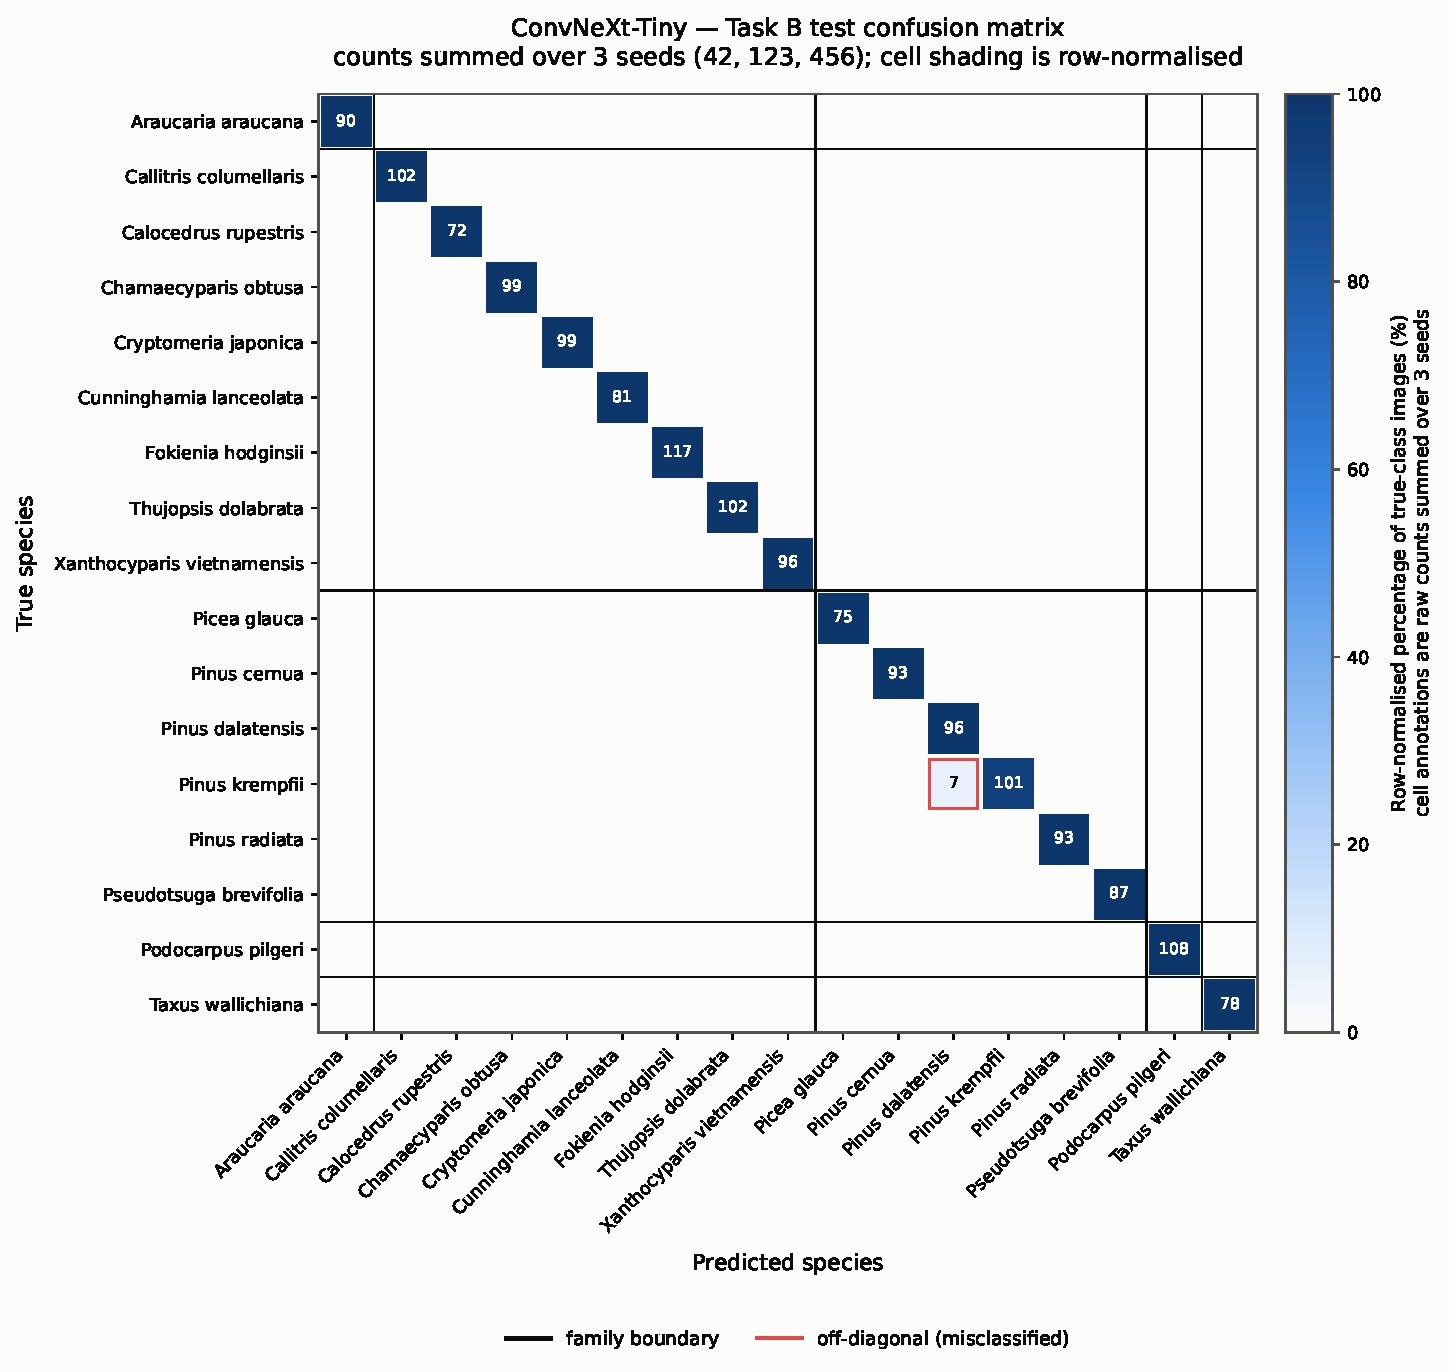
\includegraphics[width=\columnwidth]{artifact/person3/confusion/fig_confusion.pdf}
\caption{Ma trận nhầm lẫn của ConvNeXt-Tiny trên tập test Task~B. Các count được cộng theo từng phần tử qua ba seed chính (42, 123, 456), cho $532\times3 = 1{,}596$ dự đoán; mỗi seed đóng góp như nhau. Màu nền ô là tỷ lệ phần trăm đã chuẩn hóa theo hàng của số ảnh thuộc lớp thật, với mẫu số là tổng hàng của các count đã cộng; số ghi trong mỗi ô là count thô đã cộng. Các loài được sắp theo họ và các đường kẻ đen đánh dấu ranh giới họ. Ô ngoài đường chéo được viền đỏ. ConvNeXt-Tiny được chọn theo tiêu chí cố định trước (macro-F1 trung bình cao nhất trên ba seed ở Bảng~\ref{tab:task_b}), chứ không phải bằng cách xem ma trận này. Ba ma trận riêng từng seed được công bố kèm bản gộp để kiểm tra lại được phép cộng.}
\label{fig:confusion}
\end{figure}


Hình~\ref{fig:perclass} và Bảng~\ref{tab:perspecies_full} cho F1 theo từng loài
ở cả năm backbone. Ba quy luật nổi bật.

% Figure: per-species F1 by architecture (small multiples)
% Source   : docs/reports/experiments/phase_1b/final_b_new_recomputed/
%            20260819T043733Z/per_class_metrics.csv
% Artifacts: artifact/person3/per_class/{perclass_f1_summary.csv,
%            perclass_metadata.json, error_analysis.md}
% Run ids  : 15 (5 backbones x seeds 42/123/456), listed in perclass_metadata.json
\begin{figure}[!htbp]
\centering
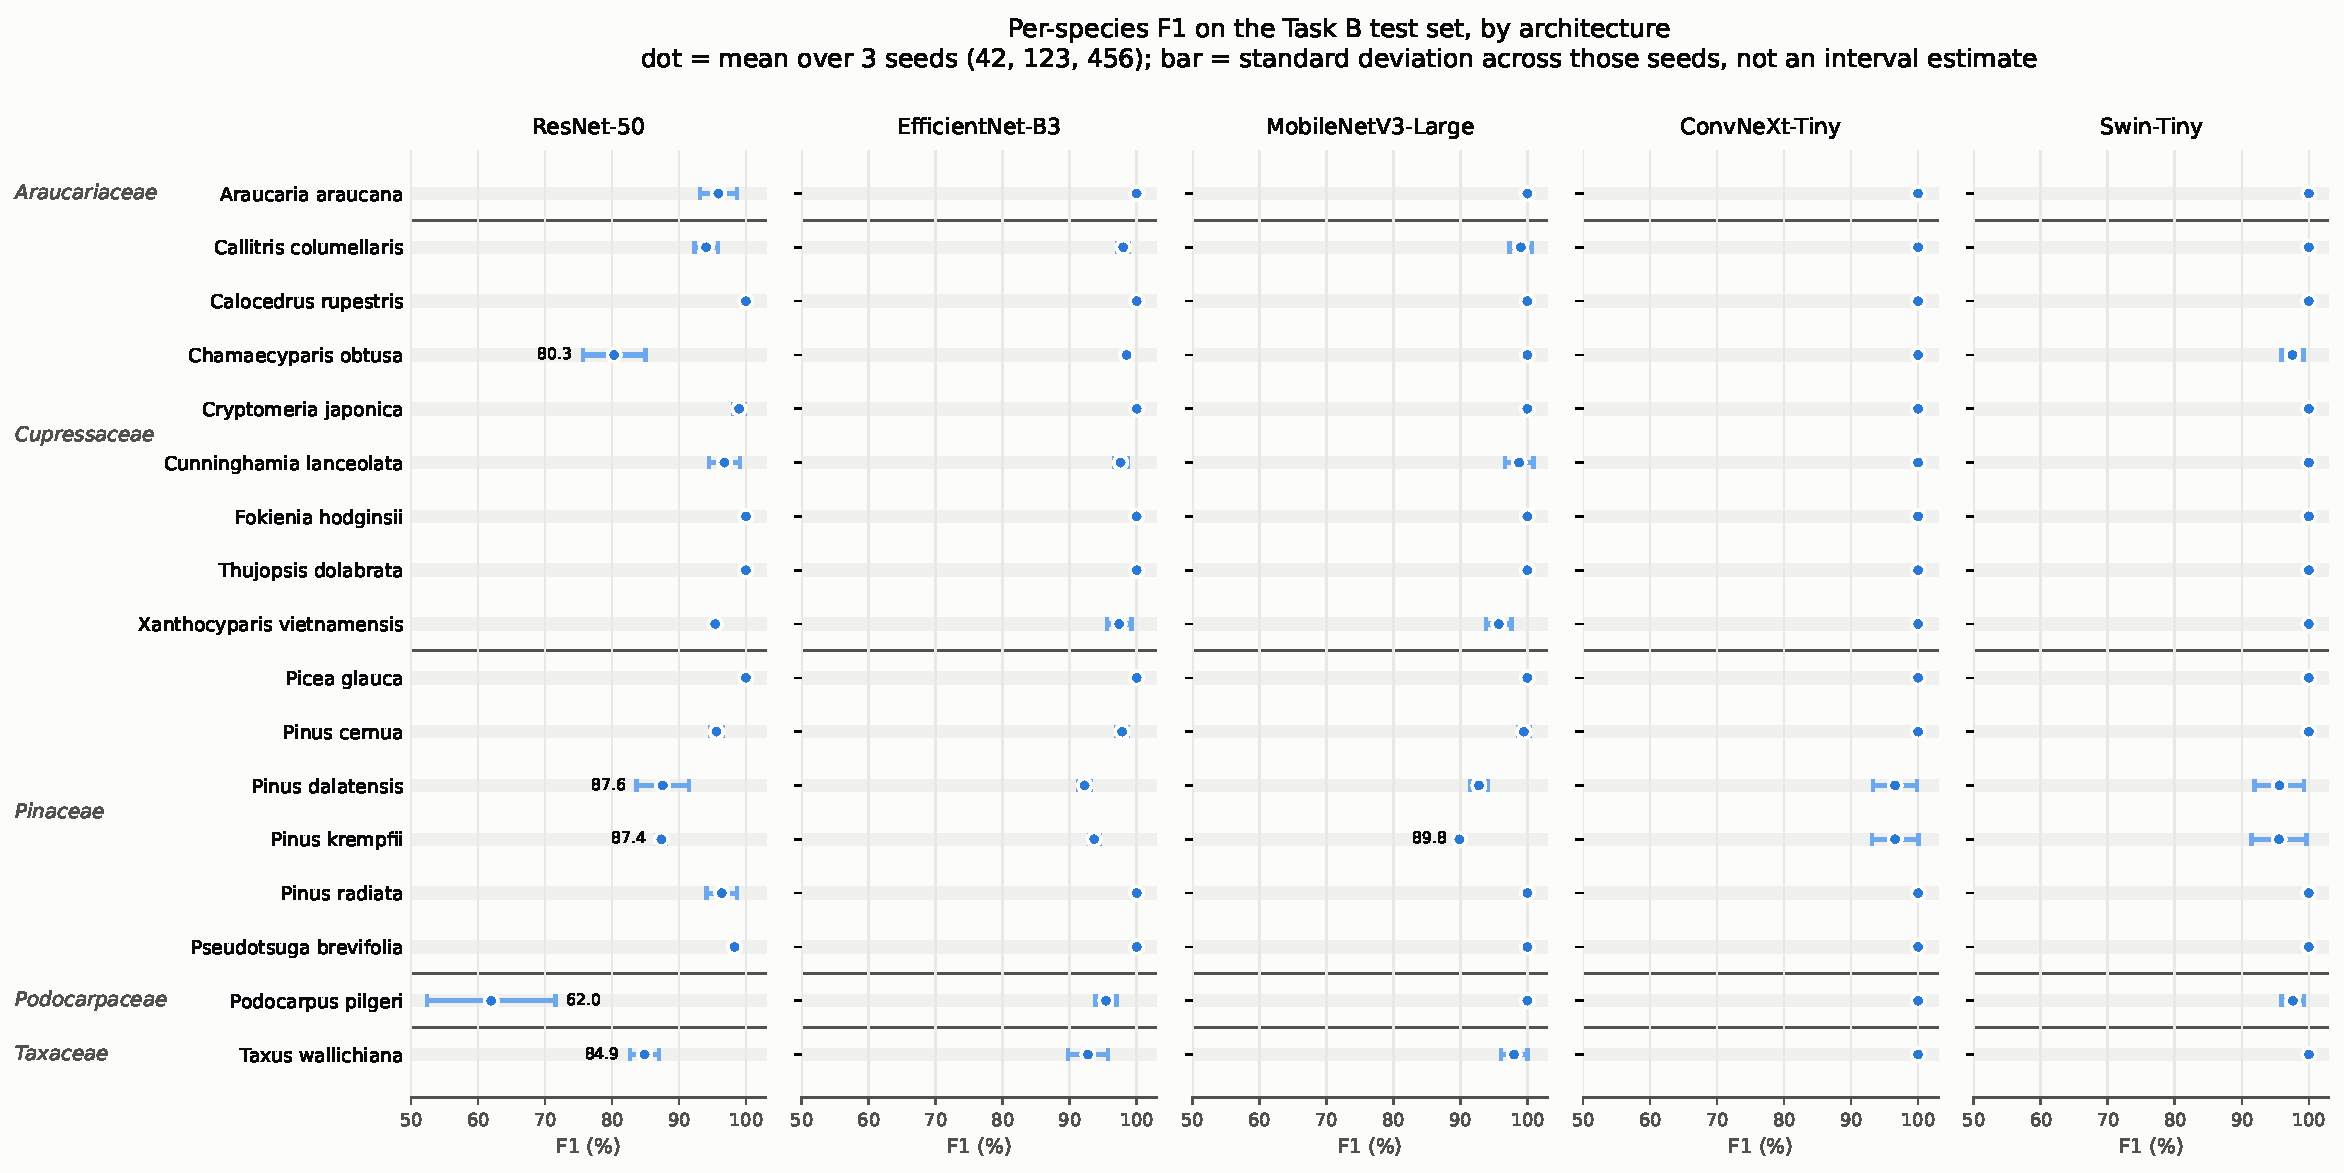
\includegraphics[width=\linewidth]{artifact/person3/per_class/fig_perclass_f1.pdf}
\caption{Điểm F1 theo từng loài trên tập test Task~B, mỗi panel một kiến trúc. Mỗi chấm là trung bình trên ba seed chính (42, 123, 456) và mỗi thanh là độ lệch chuẩn trên các seed đó; thanh này là thước đo phân tán trên ba lần chạy, không phải ước lượng khoảng. Các loài được sắp theo họ, các khối họ tách nhau bằng đường kẻ ngang và được ghi nhãn ở lề trái. Trục ngang mã hóa bằng vị trí nên không bắt đầu từ không; các giá trị dưới 90\,\% được ghi nhãn trực tiếp. Các kiến trúc được tách thành panel riêng thay vì phân biệt bằng màu, để danh tính được mang bởi vị trí và tiêu đề panel.}
\label{fig:perclass}
\end{figure}

% Table: per-species F1, full 17 classes x 5 backbones
% AUTO-GENERATED bang scripts/person3/make_result_tables.py -- khong sua tay
% Source file      : docs/reports/experiments/phase_1b/final_b_new_recomputed/20260819T043733Z/per_class_metrics.csv
% Registry created : 2026-08-19T04:37:33.586402+00:00
% Source run ids   : 15 runs
%   taskB17__main__seed_123__convnext_tiny
%   taskB17__main__seed_123__efficientnet_b3
%   taskB17__main__seed_123__mobilenetv3_large
%   taskB17__main__seed_123__resnet50
%   taskB17__main__seed_123__swin_tiny
%   taskB17__main__seed_42__convnext_tiny
%   taskB17__main__seed_42__efficientnet_b3
%   taskB17__main__seed_42__mobilenetv3_large
%   taskB17__main__seed_42__resnet50
%   taskB17__main__seed_42__swin_tiny
%   taskB17__main__seed_456__convnext_tiny
%   taskB17__main__seed_456__efficientnet_b3
%   taskB17__main__seed_456__mobilenetv3_large
%   taskB17__main__seed_456__resnet50
%   taskB17__main__seed_456__swin_tiny
\begin{table}[!htbp]
\centering
\footnotesize
\setlength{\tabcolsep}{3pt}
\caption{Điểm F1 theo từng loài (\%) trên tập test Task~B (17 loài, 532 ảnh), cho từng backbone. Giá trị là trung bình $\pm$ độ lệch chuẩn trên 3 seed huấn luyện chính (42, 123, 456); độ phân tán là độ lệch chuẩn trên ba lần chạy, không phải ước lượng khoảng. Các loài được nhóm theo họ. $n$ là số ảnh test của mỗi loài.}
\label{tab:perspecies_full}
\resizebox{\linewidth}{!}{%
\begin{tabular}{lrccccc}
\toprule
\textbf{Loài} & $n$ & \textbf{ResNet-50} & \textbf{EfficientNet-B3} & \textbf{MobileNetV3-Large} & \textbf{ConvNeXt-Tiny} & \textbf{Swin-Tiny} \\
\midrule
\multicolumn{7}{l}{\textit{Araucariaceae}} \\
\quad \textit{Araucaria araucana} & 30 & $95.905 \pm 2.781$ & $100.000 \pm 0.000$ & $100.000 \pm 0.000$ & $100.000 \pm 0.000$ & $100.000 \pm 0.000$ \\
\midrule
\multicolumn{7}{l}{\textit{Cupressaceae}} \\
\quad \textit{Callitris columellaris} & 34 & $94.067 \pm 1.734$ & $97.995 \pm 0.888$ & $99.020 \pm 1.698$ & $100.000 \pm 0.000$ & $100.000 \pm 0.000$ \\
\quad \textit{Calocedrus rupestris} & 24 & $100.000 \pm 0.000$ & $100.000 \pm 0.000$ & $100.000 \pm 0.000$ & $100.000 \pm 0.000$ & $100.000 \pm 0.000$ \\
\quad \textit{Chamaecyparis obtusa} & 33 & $80.336 \pm 4.658$ & $98.492 \pm 0.027$ & $100.000 \pm 0.000$ & $100.000 \pm 0.000$ & $97.556 \pm 1.649$ \\
\quad \textit{Cryptomeria japonica} & 33 & $98.974 \pm 0.888$ & $100.000 \pm 0.000$ & $100.000 \pm 0.000$ & $100.000 \pm 0.000$ & $100.000 \pm 0.000$ \\
\quad \textit{Cunninghamia lanceolata} & 27 & $96.781 \pm 2.307$ & $97.597 \pm 1.012$ & $98.765 \pm 2.138$ & $100.000 \pm 0.000$ & $100.000 \pm 0.000$ \\
\quad \textit{Fokienia hodginsii} & 39 & $100.000 \pm 0.000$ & $100.000 \pm 0.000$ & $100.000 \pm 0.000$ & $100.000 \pm 0.000$ & $100.000 \pm 0.000$ \\
\quad \textit{Thujopsis dolabrata} & 34 & $100.000 \pm 0.000$ & $100.000 \pm 0.000$ & $100.000 \pm 0.000$ & $100.000 \pm 0.000$ & $100.000 \pm 0.000$ \\
\quad \textit{Xanthocyparis vietnamensis} & 32 & $95.431 \pm 0.080$ & $97.387 \pm 1.861$ & $95.733 \pm 1.892$ & $100.000 \pm 0.000$ & $100.000 \pm 0.000$ \\
\midrule
\multicolumn{7}{l}{\textit{Pinaceae}} \\
\quad \textit{Picea glauca} & 25 & $100.000 \pm 0.000$ & $100.000 \pm 0.000$ & $100.000 \pm 0.000$ & $100.000 \pm 0.000$ & $100.000 \pm 0.000$ \\
\quad \textit{Pinus cernua} & 31 & $95.610 \pm 0.915$ & $97.832 \pm 0.916$ & $99.471 \pm 0.916$ & $100.000 \pm 0.000$ & $100.000 \pm 0.000$ \\
\quad \textit{Pinus dalatensis} & 32 & $87.596 \pm 3.913$ & $92.228 \pm 0.911$ & $92.767 \pm 1.345$ & $96.559 \pm 3.295$ & $95.620 \pm 3.706$ \\
\quad \textit{Pinus krempfii} & 36 & $87.383 \pm 0.738$ & $93.663 \pm 0.788$ & $89.849 \pm 0.294$ & $96.573 \pm 3.495$ & $95.548 \pm 4.082$ \\
\quad \textit{Pinus radiata} & 31 & $96.409 \pm 2.273$ & $100.000 \pm 0.000$ & $100.000 \pm 0.000$ & $100.000 \pm 0.000$ & $100.000 \pm 0.000$ \\
\quad \textit{Pseudotsuga brevifolia} & 29 & $98.305 \pm 0.000$ & $100.000 \pm 0.000$ & $100.000 \pm 0.000$ & $100.000 \pm 0.000$ & $100.000 \pm 0.000$ \\
\midrule
\multicolumn{7}{l}{\textit{Podocarpaceae}} \\
\quad \textit{Podocarpus pilgeri} & 36 & $61.994 \pm 9.598$ & $95.420 \pm 1.562$ & $100.000 \pm 0.000$ & $100.000 \pm 0.000$ & $97.612 \pm 1.697$ \\
\midrule
\multicolumn{7}{l}{\textit{Taxaceae}} \\
\quad \textit{Taxus wallichiana} & 26 & $84.891 \pm 2.182$ & $92.732 \pm 2.970$ & $98.013 \pm 2.000$ & $100.000 \pm 0.000$ & $100.000 \pm 0.000$ \\
\bottomrule
\end{tabular}}
\end{table}


\textit{Thứ nhất}, cặp \textit{P.\ krempfii} / \textit{P.\ dalatensis} là
nhầm lẫn duy nhất xuất hiện ở \emph{mọi} kiến trúc: 18, 12, 15, 9 và 7 lần lần
lượt với ResNet-50, EfficientNet-B3, MobileNetV3-Large, Swin-Tiny và
ConvNeXt-Tiny, tổng cộng 61 lần, so với đúng một lần theo chiều ngược lại. Nó
chiếm 61 trong tổng số 204 lỗi của tất cả backbone và seed cộng lại, và không
giảm đi khi năng lực mô hình tăng. Cả hai loài đều thuộc chi \textit{Pinus}
(họ Pinaceae) với số ảnh test tương đương (36 và 32), nên cả mất cân bằng lớp
lẫn ranh giới họ đều không giải thích được hiện tượng này. Hai loài này cũng
mang độ lệch chuẩn giữa các seed lớn nhất trong hai cột mạnh nhất, dao động từ 3.30
đến 4.08 điểm (so với 0 ở mọi loài còn lại dưới ConvNeXt-Tiny), nên bản thân
độ lớn của hiệu ứng cũng không ổn định.

\textit{Thứ hai}, lỗi không phân bố đều giữa các kiến trúc. Riêng ResNet-50 gây
ra 122 trong 204 lỗi. Trường hợp tệ nhất của nó là \textit{Podocarpus
pilgeri}, chỉ đạt $61.994 \pm 9.598$\,\% F1, thấp hơn mô hình kế tiếp 33.4
điểm và là ô có độ phân tán lớn nhất trong Bảng~\ref{tab:perspecies_full},
do 48 lần nhầm với \textit{Chamaecyparis obtusa}. Bốn kiến trúc còn lại đạt từ
95.420 đến 100.000\,\% F1 trên \emph{cùng} bộ ảnh đó, và hai trong số đó không
mắc lỗi này lần nào. Nếu gộp chung các kiến trúc thì cặp này sẽ hiện ra như
khó khăn lớn thứ hai của bộ dữ liệu; khi tách riêng, nó gần như hoàn toàn là
chế độ thất bại của một mô hình trên cấu hình này, chứ không phải bằng chứng
rằng hai loại gỗ giống nhau.

\textit{Thứ ba}, độ khó ở cấp họ không theo trực giác rằng họ lớn nhất là họ
khó nhất. Tỷ lệ lỗi của từng họ lần lượt là 1.56\,\% với Araucariaceae,
0.78\,\% với Cupressaceae, 2.83\,\% với Pinaceae, 10.93\,\% với
Podocarpaceae và 7.69\,\% với Taxaceae. Cupressaceae, họ lớn nhất với tám
loài, là họ \emph{thấp nhất} trong năm, và cả tám loài đều không có lỗi nào
dưới ConvNeXt-Tiny. Ba trong năm họ chỉ chứa đúng một loài (Araucariaceae,
Podocarpaceae, Taxaceae), nên tỷ lệ của chúng là tỷ lệ một loài trên mẫu số nhỏ
hơn hẳn và không so sánh cùng loại với tỷ lệ của họ tám loài và họ sáu loài.
Loại ResNet-50 khỏi phép tính lại làm đổi thứ tự này một lần nữa: Araucariaceae
giảm còn 0.00\,\%, Podocarpaceae còn 2.08\,\% và Taxaceae còn 3.53\,\%,
trong khi Cupressaceae đạt 0.49\,\% và Pinaceae đạt 2.13\,\%. Như vậy ba
trong năm họ có độ khó biểu kiến chủ yếu đến từ một backbone duy nhất, và thứ
tự giữa các họ còn lại không ổn định giữa hai cách nhóm.

\subsection{Xoay ảnh và label smoothing}
\label{vi:sec:results:ablation}

Bảng~\ref{tab:ablation} báo cáo ba ablation, đối chiếu với cấu hình chính ở
\emph{cùng seed và cùng backbone}: xoay rời rạc $90^\circ$ thay cho xoay liên
tục $\pm30^\circ$, và label smoothing đặt về 0.0 rồi 0.2 thay cho 0.1. Mỗi
ablation chỉ huấn luyện với seed 42, nên mỗi ô trong bảng là một ước lượng
điểm từ một lần chạy duy nhất, không có độ phân tán riêng.

% Table: Task B ablations vs main seed 42 (same backbone)
% LUU Y: moi ablation chi co 1 seed (42) -> khong co +/- , chi la diem don.
% AUTO-GENERATED bang scripts/person3/make_result_tables.py -- khong sua tay
% Source file      : docs/reports/experiments/phase_1b/final_b_new_recomputed/20260819T043733Z/ablation_vs_main_seed42.csv
% Registry created : 2026-08-19T04:37:33.586402+00:00
% Source run ids   : 15 runs
%   taskB17__taskB_90rotation__seed_42__convnext_tiny
%   taskB17__taskB_90rotation__seed_42__efficientnet_b3
%   taskB17__taskB_90rotation__seed_42__mobilenetv3_large
%   taskB17__taskB_90rotation__seed_42__resnet50
%   taskB17__taskB_90rotation__seed_42__swin_tiny
%   taskB17__taskB_label_smoothing_0p0__seed_42__convnext_tiny
%   taskB17__taskB_label_smoothing_0p0__seed_42__efficientnet_b3
%   taskB17__taskB_label_smoothing_0p0__seed_42__mobilenetv3_large
%   taskB17__taskB_label_smoothing_0p0__seed_42__resnet50
%   taskB17__taskB_label_smoothing_0p0__seed_42__swin_tiny
%   taskB17__taskB_label_smoothing_0p2__seed_42__convnext_tiny
%   taskB17__taskB_label_smoothing_0p2__seed_42__efficientnet_b3
%   taskB17__taskB_label_smoothing_0p2__seed_42__mobilenetv3_large
%   taskB17__taskB_label_smoothing_0p2__seed_42__resnet50
%   taskB17__taskB_label_smoothing_0p2__seed_42__swin_tiny
% Baseline run ids : 5 runs
%   taskB17__main__seed_42__convnext_tiny
%   taskB17__main__seed_42__efficientnet_b3
%   taskB17__main__seed_42__mobilenetv3_large
%   taskB17__main__seed_42__resnet50
%   taskB17__main__seed_42__swin_tiny
\begin{table}[!htbp]
\centering
\footnotesize
\setlength{\tabcolsep}{3pt}
\caption{Ảnh hưởng của từng ablation lên hiệu năng test Task~B, đối chiếu với cấu hình chính ở \emph{cùng seed và cùng backbone}. Hai cột trái cho điểm tuyệt đối của lần chạy chính với seed 42; mỗi cột $\Delta$ là ablation trừ đi lần chạy chính cùng backbone, tính bằng điểm phần trăm. Mỗi ablation chỉ huấn luyện với một seed (42), nên không ước lượng được độ phân tán cho các lần chạy này và các chênh lệch dưới đây là ước lượng điểm từ một lần chạy chứ không phải hiệu ứng đã lấy trung bình. Để đối chiếu, độ lệch chuẩn giữa các seed của các lần chạy chính ở Bảng~\ref{tab:task_b} có độ lớn tương đương với phần lớn các chênh lệch này.}
\label{tab:ablation}
\begin{tabular}{lcccccccc}
\toprule
\textbf{Kiến trúc} & \multicolumn{2}{c}{\textbf{Chính (seed 42)}} & \multicolumn{2}{c}{\textbf{Xoay rời rạc $90^\circ$}} & \multicolumn{2}{c}{\textbf{Label smoothing $0.0$}} & \multicolumn{2}{c}{\textbf{Label smoothing $0.2$}} \\
\cmidrule(lr){2-3} \cmidrule(lr){4-5} \cmidrule(lr){6-7} \cmidrule(lr){8-9}
 & Acc.\ (\%) & F1 (\%) & $\Delta$Acc. & $\Delta$F1 & $\Delta$Acc. & $\Delta$F1 & $\Delta$Acc. & $\Delta$F1 \\
\midrule
ResNet-50         & $93.797$ & $93.944$ & $+0.940$ & $+0.743$ & $-0.376$ & $-0.316$ & $+0.564$ & $+0.557$ \\
EfficientNet-B3   & $97.368$ & $97.405$ & $+1.316$ & $+1.299$ & $-0.752$ & $-0.795$ & $-0.376$ & $-0.415$ \\
MobileNetV3-Large & $98.684$ & $98.787$ & $+0.000$ & $+0.000$ & $-0.376$ & $-0.369$ & $+0.000$ & $+0.000$ \\
ConvNeXt-Tiny     & $99.812$ & $99.827$ & $-0.564$ & $-0.519$ & $-0.188$ & $-0.187$ & $-0.752$ & $-0.689$ \\
Swin-Tiny         & $99.624$ & $99.656$ & $-0.564$ & $-0.521$ & $-0.188$ & $-0.175$ & $-0.188$ & $-0.198$ \\
\bottomrule
\end{tabular}
\end{table}


Xoay rời rạc $90^\circ$ không tạo ra hiệu ứng nhất quán. Các chênh lệch độ
chính xác lần lượt là $+0.940$, $+1.316$, $0.000$, $-0.564$ và $-0.564$ điểm
phần trăm cho ResNet-50, EfficientNet-B3, MobileNetV3-Large, ConvNeXt-Tiny và
Swin-Tiny, trong đó giá trị dương với hai backbone tích chập yếu hơn, bằng không với một, và
âm với cả hai mô hình mạnh nhất. Dấu của hiệu ứng không ổn định giữa các kiến
trúc, và bốn trong năm độ lớn nằm trong khoảng 1.6 lần độ lệch chuẩn giữa các
seed tương ứng ở Bảng~\ref{tab:task_b}. Chỉ EfficientNet-B3 có chênh lệch rõ
ràng lớn hơn nhiễu tạp âm seed của chính nó, khoảng bốn lần độ lệch chuẩn, và
với một seed thì không thể tách nó khỏi một lần bốc may mắn.

Bỏ hẳn label smoothing ($0.0$) làm giảm độ chính xác ở \emph{cả năm} backbone:
$-0.376$, $-0.752$, $-0.376$, $-0.188$ và $-0.188$ điểm phần trăm. Từng độ lớn
đều nhỏ (ba trong năm giá trị nằm dưới độ lệch chuẩn giữa các seed tương ứng),
nhưng hướng của hiệu ứng giống nhau ở cả năm trường hợp, và đây là quy luật
nhất quán duy nhất trong bảng ablation. Nâng label smoothing lên $0.2$ không
cho sự nhất quán như vậy: hai backbone tăng hoặc giữ nguyên, ba backbone giảm.

Gộp lại, không ablation nào đủ căn cứ để đưa ra khuyến nghị. Kết quả xoay ảnh
phản bác việc coi tăng cường $90^\circ$ rời rạc là một cải tiến phổ quát cho
bài toán này, còn phép quét label smoothing gợi ý rằng giá trị mặc định 0.1 ít
nhất không tệ hơn hai giá trị lân cận đã thử. Cả hai cách đọc đều bị giới hạn
bởi thiết kế một seed (Mục~\ref{vi:sec:discussion:oneseed}).

\subsection{Sự hội tụ và tính đủ của thông tin giải phẫu}
\label{vi:sec:results:convergence}

\paragraph{Hội tụ.} Đường cong theo từng epoch không được lưu lại cho các lần
chạy trong registry, nên sự hội tụ được mô tả qua các trường tóm tắt ghi kèm
mỗi checkpoint. Hai backbone mạnh nhất hội tụ trong khoảng một phần ba ngân
sách: epoch validation tốt nhất trung bình là 20.3 với ConvNeXt-Tiny và 15.0
với Swin-Tiny, so với 40.3--44.0 với MobileNetV3-Large, EfficientNet-B3 và
ResNet-50. Dừng sớm (early stopping) kích hoạt ở cả ba seed với ConvNeXt-Tiny
và Swin-Tiny, và không lần nào với ResNet-50. Khoảng cách giữa độ chính xác
train cuối và validation cuối tách đúng hai nhóm đó: 0.17 và 0.48 điểm với
ConvNeXt-Tiny và Swin-Tiny, so với 3.14, 3.85 và 4.73 với ba mô hình còn lại.
Như vậy thứ tự theo tốc độ hội tụ và theo khoảng cách khái quát hóa trùng với
thứ tự theo độ chính xác test ở Bảng~\ref{tab:task_b}.

\paragraph{Tính đủ của thông tin giải phẫu.} Một thí nghiệm đối chứng kiểm tra
xem bài toán có thật sự đòi hỏi chi tiết giải phẫu hay không. Ba phép thăm dò
được huấn luyện trên cùng phân hoạch và đánh giá một lần trên cùng tập test:
\textbf{B1}, ảnh hạ xuống $16\times16$ rồi phóng lại $224\times224$;
\textbf{B2}, ảnh làm mờ Gaussian với nhân kích thước 49 và $\sigma=8$; và
\textbf{B3}, một mạng perceptron nhiều lớp nhỏ chỉ nhận histogram RGB
$3\times32$ bin đã chuẩn hóa, tức bỏ toàn bộ cấu trúc không gian. B1 và B2 dùng
Swin-Tiny khởi tạo mới từ ImageNet; mức tham chiếu toàn ảnh là lần chạy
Swin-Tiny tương ứng, đạt 99.060\,\% độ chính xác.

\begin{table}[htbp]
\centering
\small
\caption{Ba phép thăm dò phá hủy cấu trúc giải phẫu, đánh giá một lần trên
cùng tập test Task~B với cùng phân hoạch. Cột \emph{Giữ lại} là tỷ lệ phần
trăm độ chính xác so với mức tham chiếu toàn ảnh. Nguồn: thư mục thăm dò
\texttt{anatomy\_destruction\_probe} của cùng đợt thực nghiệm phase~1b.}
\label{tab:probe}
\begin{tabular}{llcc}
\toprule
\textbf{Phép thăm dò} & \textbf{Đầu vào} & \textbf{Độ chính xác (\%)} & \textbf{Giữ lại (\%)} \\
\midrule
Ngẫu nhiên đều     & không ảnh                & 5.882  & --- \\
Lớp đa số          & không ảnh                & 7.331  & --- \\
Ảnh đầy đủ         & $224\times224$           & 99.060 & 100.0 \\
B1                 & $16\times16$ phóng lại    & 94.361 & 95.3 \\
B2                 & làm mờ $\sigma=8$        & 95.677 & 96.6 \\
B3                 & chỉ histogram RGB        & 37.970 & 38.3 \\
\bottomrule
\end{tabular}
\end{table}

Ở mức $16\times16$, mọi cấu trúc mà một nhà giải phẫu gỗ dùng đến (như đường
kính quản bào, ống nhựa, tế bào tia, ranh giới vòng năm) đều bị phá hủy,
vậy mà độ chính xác vẫn giữ được 95.3\,\% so với mức tham chiếu toàn ảnh. Làm
mờ nặng giữ được 96.6\,\%. Riêng màu sắc không đủ: B3 chỉ đạt 37.970\,\%, cao
hơn hẳn mức ngẫu nhiên 5.882\,\% nhưng thấp hơn nhiều so với cả hai phép thăm
dò có thông tin không gian. Như vậy bài toán ở dạng hiện tại phần lớn giải
được bằng nội dung ảnh tần số thấp, thành phần còn lại sau khi phá hủy chi tiết
giải phẫu, và các mức độ chính xác quanh $99$\,\% ở Bảng~\ref{tab:task_b}
\textbf{không thể đọc như bằng chứng rằng mô hình đang định danh gỗ bằng giải
phẫu}. Mục~\ref{vi:sec:discussion:shortcut} bàn tiếp về hệ quả của điều này.

\subsection{Độ phức tạp mô hình}
\label{vi:sec:results:efficiency}

Bảng~\ref{tab:efficiency} báo cáo số tham số, số phép nhân-cộng (MACs) và kích
thước mô hình ở độ phân giải đầu vào $224\times224$.

% Table: model complexity (params / MACs / size)
% AUTO-GENERATED bang scripts/person3/make_result_tables.py -- khong sua tay
% Source file      : results/efficiency.csv
% KHONG thuoc registry 20260819T043733Z: day la thuoc tinh kien truc,
% do voi pretrained=False nen doc lap voi checkpoint va lan huan luyen.
% Latency da BO (do tren NVIDIA GeForce RTX 3060, khac phan cung cua registry).
% Cot MACs = cot flops_g cua CSV chia 2 (CSV dem FLOPs = 2 x MACs).
\begin{table}[!htbp]
\centering
\caption{Độ phức tạp của năm kiến trúc ở độ phân giải đầu vào $224\times224$ dùng xuyên suốt, với đầu ra 17 lớp. Số tham số, số phép nhân cộng (MACs) và kích thước mô hình là thuộc tính của kiến trúc: chúng được đo trên mô hình khởi tạo ngẫu nhiên và không phụ thuộc vào bất kỳ checkpoint đã huấn luyện nào. Báo cáo MACs thay vì FLOPs; script đo ghi $\text{FLOPs} = 2\times\text{MACs}$, và các giá trị dưới đây là cột đó chia đôi, để so sánh trực tiếp được với quy ước dùng trong tài liệu về kiến trúc. Độ trễ suy luận không được báo cáo: nó đo trên phần cứng khác với phần cứng huấn luyện và đánh giá, nên không so sánh được với bất kỳ con số nào khác trong bài.}
\label{tab:efficiency}
\begin{tabular}{lccc}
\toprule
\textbf{Kiến trúc} & \textbf{Tham số (M)} & \textbf{MACs (G)} & \textbf{Kích thước (MB)} \\
\midrule
ResNet-50         & $23.54$ & $4.13$ & $90.11$ \\
EfficientNet-B3   & $10.72$ & $0.94$ & $41.42$ \\
MobileNetV3-Large & $4.22$ & $0.22$ & $16.30$ \\
ConvNeXt-Tiny     & $27.83$ & $4.46$ & $106.24$ \\
Swin-Tiny         & $27.53$ & $4.37$ & $105.09$ \\
\bottomrule
\end{tabular}
\end{table}


Thứ hạng độ chính xác không đi theo kích thước mô hình. MobileNetV3-Large đạt
$98.371 \pm 0.319$\,\% (Bảng~\ref{tab:task_b}) với 4.22\,M tham số và
0.22\,G MACs, tương đương khoảng một phần sáu số tham số và một phần hai mươi khối
lượng tính toán của ConvNeXt-Tiny, đổi lại chênh lệch 1.19 điểm độ chính xác.
ResNet-50, với 23.54\,M tham số và 4.13\,G MACs, chỉ kém ConvNeXt-Tiny 15\,\%
khối lượng tính toán nhưng thấp hơn bảy điểm, nên khoảng cách giữa hai mô hình
này không giải thích được bằng năng lực. ConvNeXt-Tiny và Swin-Tiny gần như
giống hệt nhau về độ phức tạp (27.83 so với 27.53\,M tham số, 4.46 so với
4.37\,G MACs), khiến chênh lệch độ chính xác giữa chúng là một phép so sánh về
kiến trúc chứ không phải về quy mô.

Bảng này có hai giới hạn. Độ trễ suy luận không được báo cáo: các phép đo có
sẵn được thực hiện trên phần cứng khác với phần cứng huấn luyện và đánh giá,
nên không thể đặt cạnh bất kỳ con số nào khác trong bài. Và các chỉ số độ phức
tạp là thuộc tính của kiến trúc, đo trên mô hình khởi tạo ngẫu nhiên, nên khác
với mọi bảng còn lại ở đây, chúng không bắt nguồn từ registry đánh giá.

\subsection{Grad-CAM và cấu trúc không gian đặc trưng}
\label{vi:sec:results:gradcam}

\paragraph{Grad-CAM.} Hình~\ref{fig:gradcam} trình bày bản đồ Grad-CAM cho
ConvNeXt-Tiny, Swin-Tiny và MobileNetV3-Large trên năm ảnh test. Các ảnh được
chọn theo một quy tắc cố định trước: trong số những ảnh mà cả ba mô hình đều
phân loại đúng, lấy ảnh gần nhất với mức độ tin cậy trung vị của ConvNeXt-Tiny
trong họ của nó, phá hòa bằng đường dẫn ảnh. Không ảnh nào được chọn vì
heatmap trông đẹp. Cả ba bản đồ đều lấy từ checkpoint seed 42 của chính những
lần chạy ở Bảng~\ref{tab:task_b}.

% Figure: Grad-CAM, 3 architectures x 5 test images
% Source   : artifact/person1/gradcam/  (repo ManifoldsTeam/WoodID, branch p1,
%            commit d39a3f6b2cc5942e1e718c0dca86e89b0d81eb4d; see SOURCE.txt)
% Checkpoints: seed-42 runs of the same registry used elsewhere in this paper
% Manifest : artifact/person1/gradcam/{gradcam_manifest.csv,
%            sample_selection.csv, gradcam_metadata.json}
%
% NOTE ON ROW LABELS. The row labels printed in the figure follow botanical
% family and therefore show Araucariaceae for Araucaria araucana. This paper
% uses the four-family scheme of docs/references/WoodID_plan.md, in which that
% species is grouped with Pinaceae. The caption below names rows by species to
% avoid the clash; the figure itself should be regenerated with four-family
% labels before submission.
\begin{figure}[!htbp]
\centering
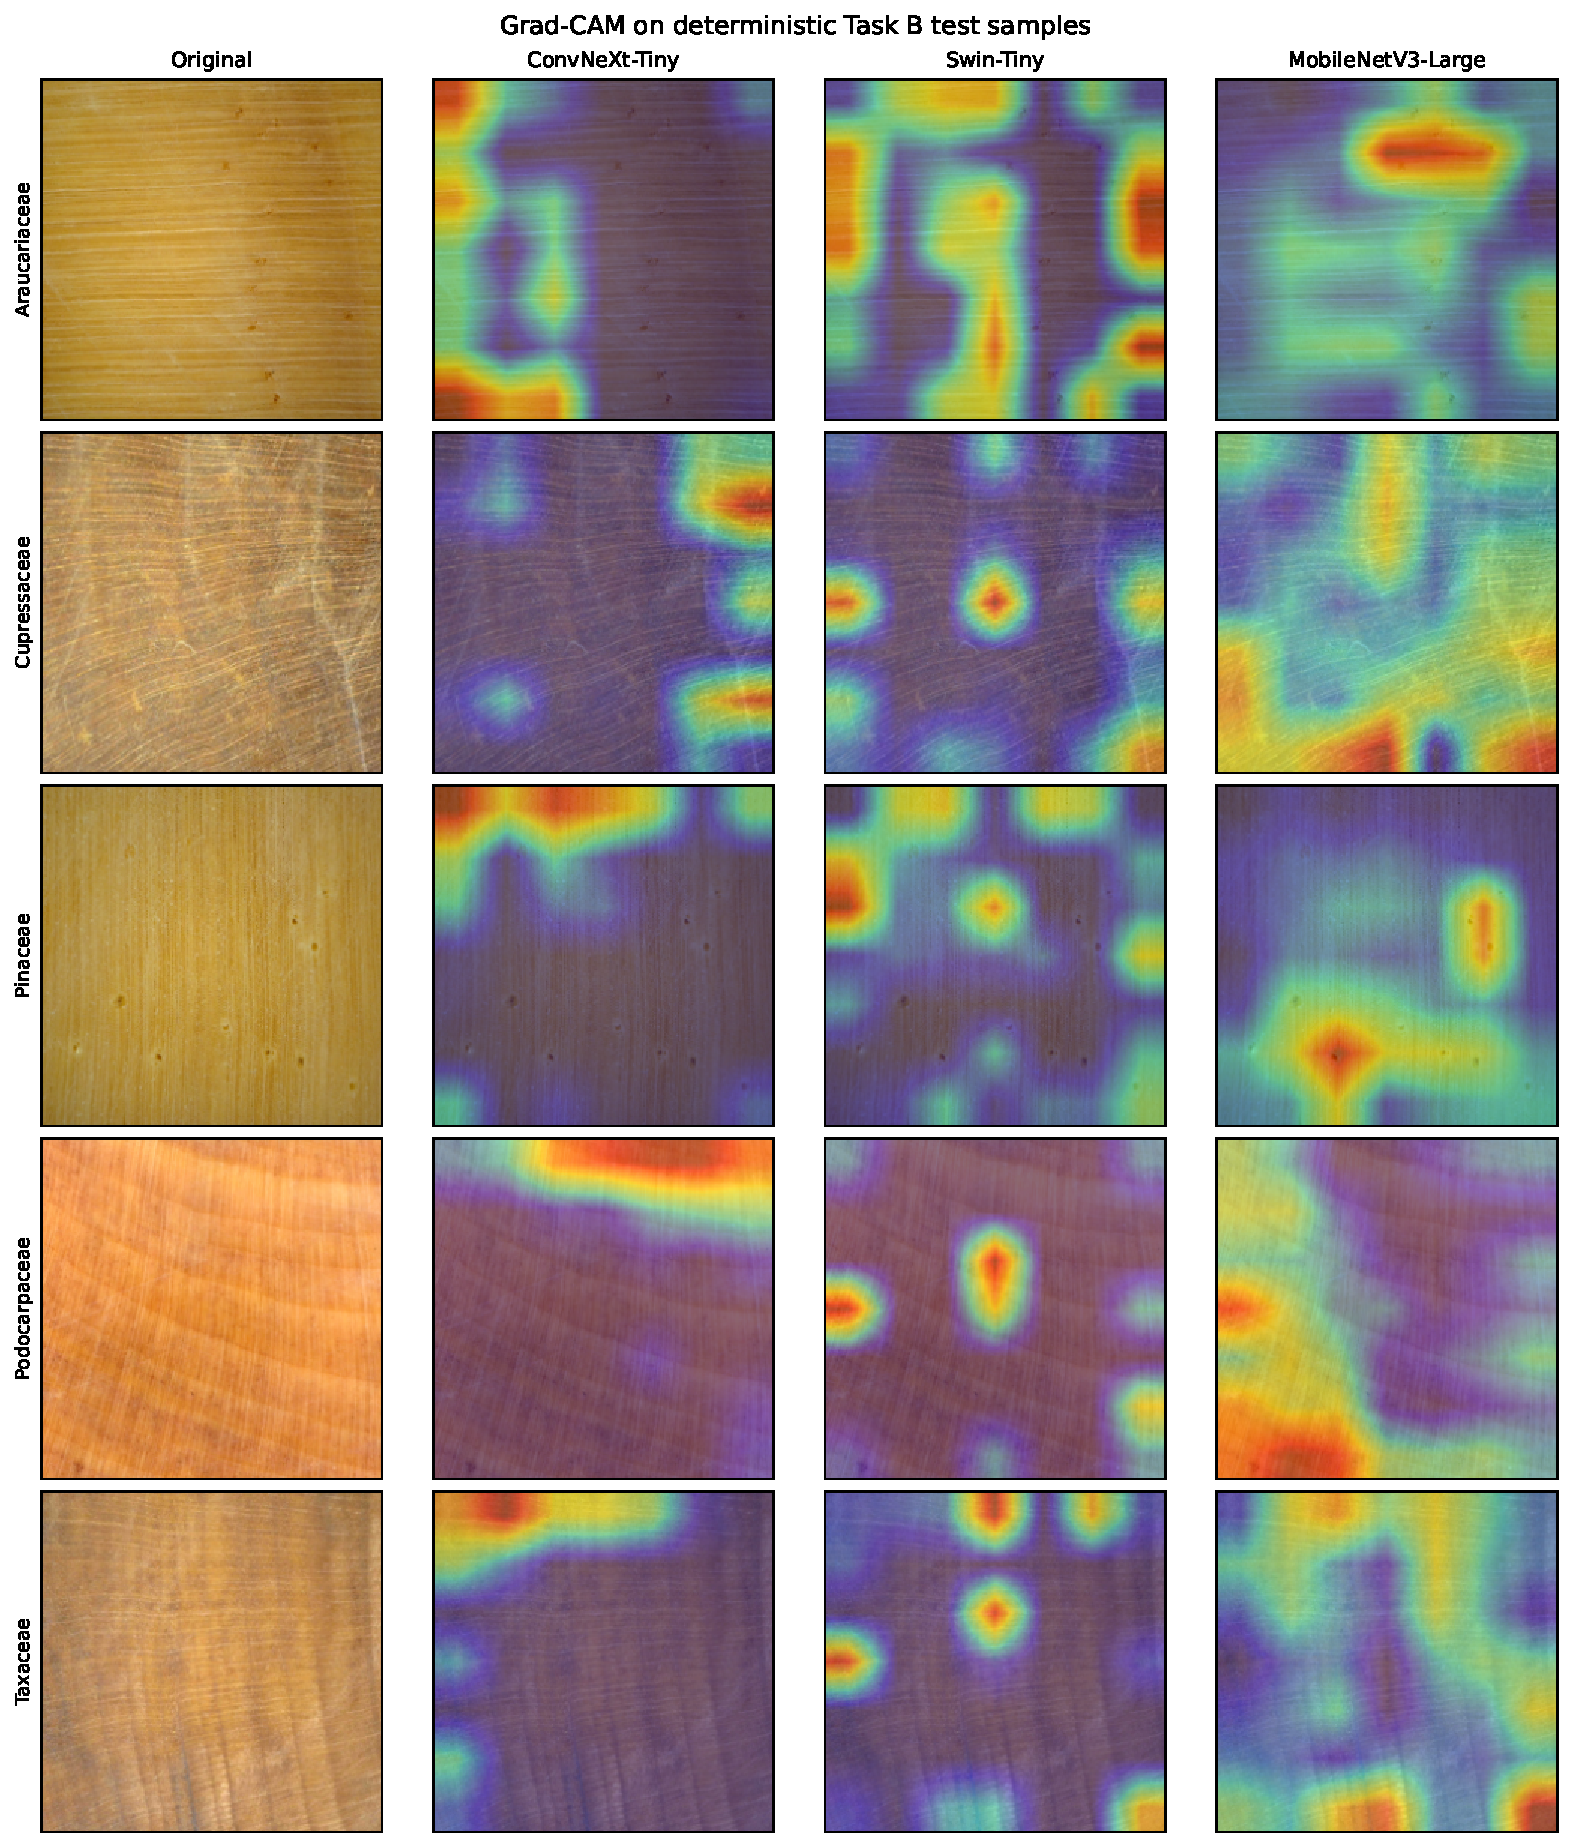
\includegraphics[width=\columnwidth]{artifact/person1/gradcam/fig_gradcam.pdf}
\caption{Bản đồ Grad-CAM cho ConvNeXt-Tiny, Swin-Tiny và MobileNetV3-Large trên năm ảnh test Task~B, mỗi họ một ảnh: \textit{Araucaria araucana}, \textit{Calocedrus rupestris}, \textit{Pinus radiata}, \textit{Podocarpus pilgeri} và \textit{Taxus wallichiana}. Ảnh được chọn theo quy tắc cố định trước: trong số những ảnh cả ba mô hình đều phân loại đúng, lấy ảnh gần nhất với mức độ tin cậy trung vị của ConvNeXt-Tiny trong họ của nó, phá hòa bằng đường dẫn ảnh. Không ảnh nào được chọn vì heatmap trông đẹp. Mỗi bản đồ đều lấy từ checkpoint seed 42 của các lần chạy ở Bảng~\ref{tab:task_b}. Các vùng quy gán trải rộng và ba kiến trúc làm nổi bật những vùng khác nhau trên cùng một ảnh; Grad-CAM định vị nơi gradient tựa vào và tự nó không xác định được đặc trưng nào đang được sử dụng.}
\label{fig:gradcam}
\end{figure}


Các vùng quy gán (attribution) trải rộng và phân tán trên khắp khung ảnh chứ
không tập trung vào những mốc giải phẫu nhận dạng được, và ba kiến trúc làm
nổi bật những vùng khác nhau trên cùng một ảnh. Đọc cùng với các phép thăm dò
ở Mục~\ref{vi:sec:results:convergence}, đây đúng là điều ta chờ đợi nếu bằng
chứng quyết định là tín hiệu tần số thấp trải đều trên ảnh chứ không phải đặc
trưng giải phẫu cục bộ. Grad-CAM cho biết gradient tựa vào đâu. Tự nó không xác
định được đặc trưng nào đang được sử dụng, và ở đây không đưa ra bất kỳ
cách đọc giải phẫu nào cho các bản đồ này.

\paragraph{Không gian đặc trưng.} Hình~\ref{fig:tsne} nhúng đặc trưng 768 chiều
trước lớp logit của ConvNeXt-Tiny seed 42 cho cả 532 ảnh test, giảm chiều bằng
PCA xuống 50 rồi bằng t-SNE xuống hai, với perplexity 30 và seed ngẫu nhiên cố
định. Các loài tạo thành những cụm phần lớn tách biệt, phù hợp với ma trận
nhầm lẫn gần như đường chéo ở Hình~\ref{fig:confusion}. Cấu trúc đáng chú ý
cho việc diễn giải là quan hệ giữa \textit{Pinus krempfii} và \textit{Pinus
dalatensis}, cặp duy nhất còn tồn tại ở mô hình tốt nhất
(Mục~\ref{vi:sec:results:perspecies}).

% Figure: t-SNE of ConvNeXt-Tiny pre-logit features, Task B test split
% Source   : artifact/person1/tsne/  (repo ManifoldsTeam/WoodID, branch p1,
%            commit d39a3f6b2cc5942e1e718c0dca86e89b0d81eb4d; see SOURCE.txt)
% Run id   : taskB17__main__seed_42__convnext_tiny  (same registry as Table 1)
% Artifacts: features_convnext_seed42_test.npz, tsne_embedding.csv,
%            tsne_metadata.json
\begin{figure}[!htbp]
\centering
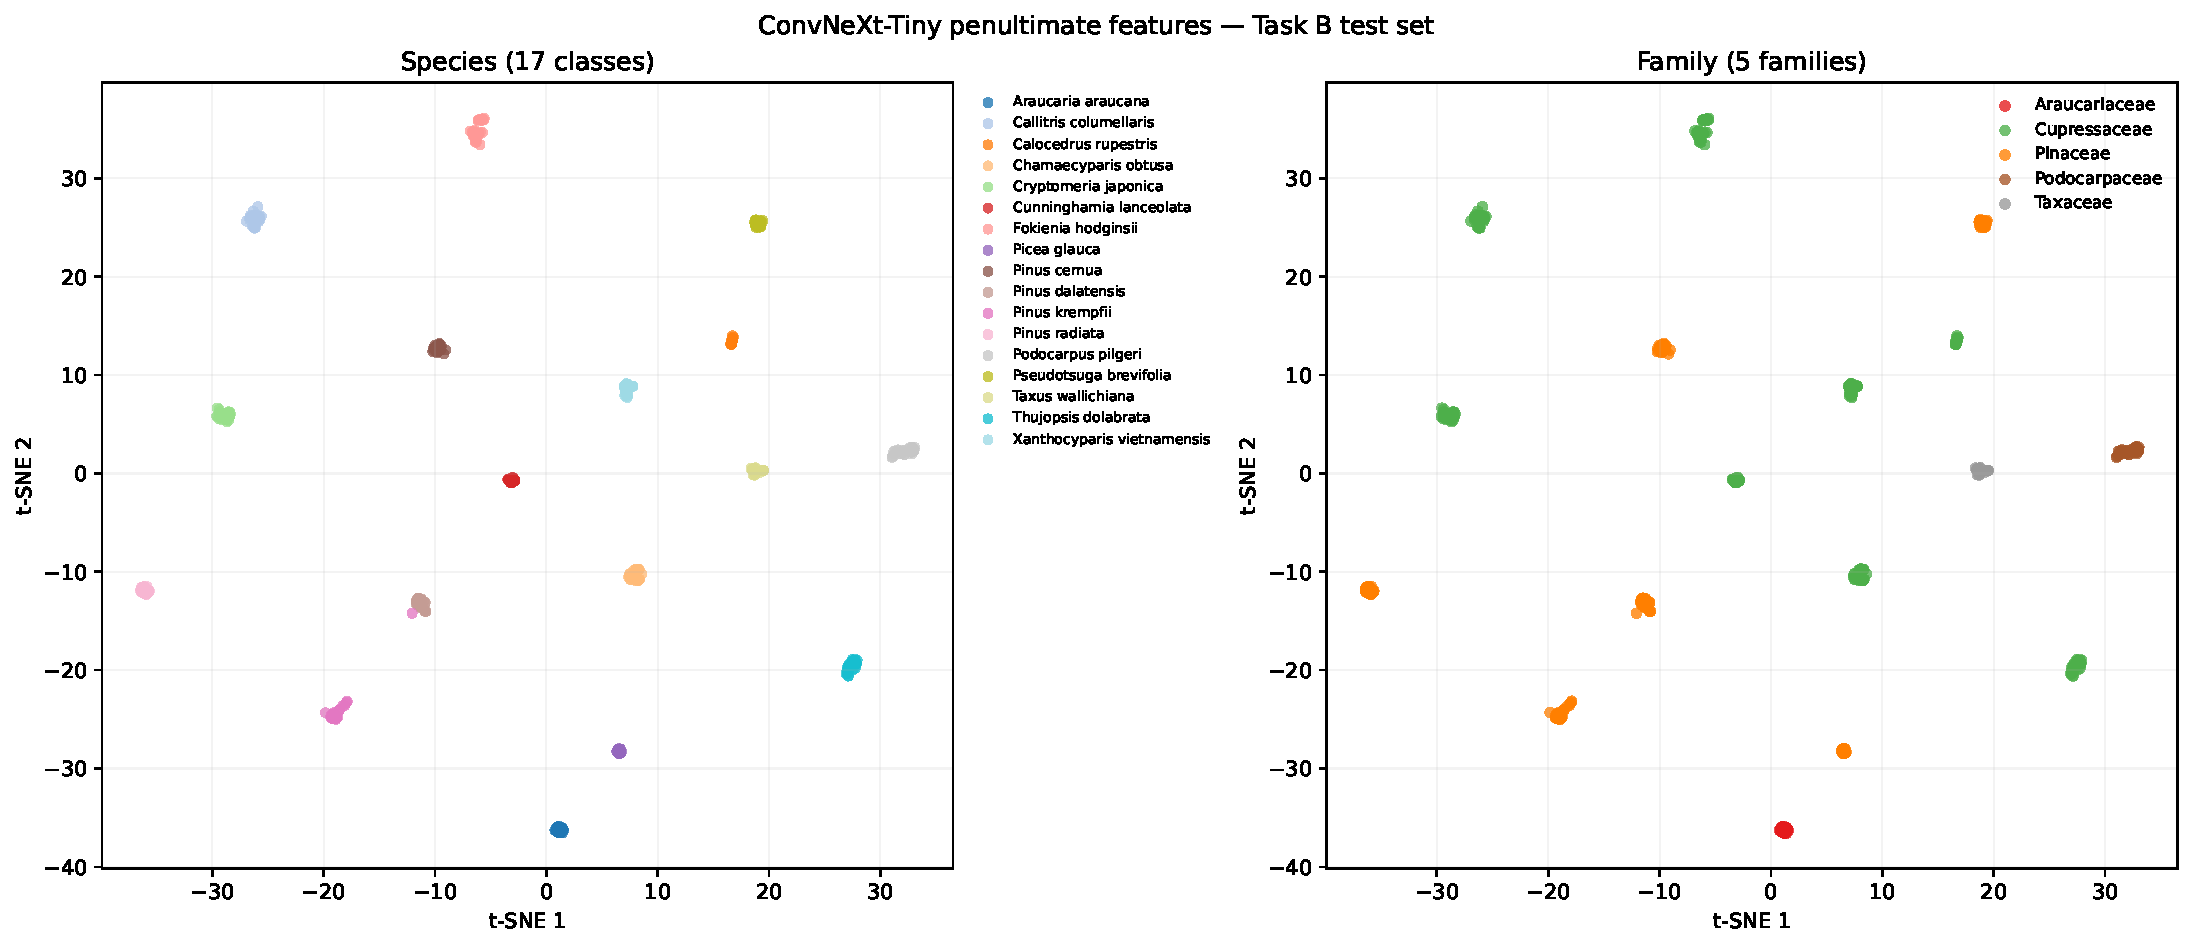
\includegraphics[width=\linewidth]{artifact/person1/tsne/fig_tsne.pdf}
\caption{Phép nhúng t-SNE hai chiều của đặc trưng ConvNeXt-Tiny cho cả 532 ảnh test Task~B, lấy từ lần chạy seed 42 ở Bảng~\ref{tab:task_b}. Đặc trưng là kích hoạt 768 chiều trước lớp logit, được chuẩn hóa, giảm xuống 50 chiều bằng PCA rồi xuống hai chiều bằng t-SNE với perplexity 30, khởi tạo PCA và seed ngẫu nhiên cố định. t-SNE chỉ bảo toàn láng giềng cục bộ: khoảng cách và diện tích cụm trong hình không phải metric, và phép nhúng được trình bày như một cách nhìn định tính về biểu diễn chứ không phải bằng chứng về tính tách được.}
\label{fig:tsne}
\end{figure}


Phép nhúng này là một phép chiếu được chọn để bảo toàn láng giềng cục bộ, và
khoảng cách trong đó không phải là metric. Phép nhúng được đưa vào như một
cách nhìn định tính về biểu diễn, không phải làm bằng chứng về tính tách được.

% =====================================================================
% Mục 5 — Bàn luận  (BẢN TIẾNG VIỆT)
%
% Bản dịch đối ứng 1-1 với sections/05_discussion.tex. Mọi con số phải giống
% bản tiếng Anh. Mục này không đưa ra con số mới nào ngoài Mục 4.
%
% Độ phân tán luôn là độ lệch chuẩn trên ba seed, không bao giờ là ước lượng
% khoảng.
%
% DẤU THẬP PHÂN: giữ dấu chấm như bản tiếng Anh, để phép kiểm tra trùng khớp
% tập con số giữa hai bản còn hiệu lực.
% =====================================================================

\section{Bàn luận}
\label{vi:sec:discussion}

\subsection{Thứ hạng kiến trúc và biến động giữa các seed}
\label{vi:sec:discussion:ranking}

Benchmark tách ra thành hai phát hiện có độ vững chắc rất khác nhau, và không
nên báo cáo chung với cùng một mức tự tin.

Phát hiện vững chắc là ResNet-50 không cạnh tranh được ở bài toán này. Mức
$92.356 \pm 1.022$\,\% của nó thấp hơn ConvNeXt-Tiny khoảng bảy điểm, một
khoảng cách gấp nhiều lần độ lệch chuẩn giữa các seed của chính nó, và nó gây
ra 122 trong 204 lỗi của cả năm backbone trên mọi seed
(Mục~\ref{vi:sec:results:perspecies}). Khoảng cách này còn mang tính cấu trúc
chứ không khuếch tán: nó tập trung ở một số loài cụ thể mà bốn kiến trúc kia
gần như hoàn hảo.

Phát hiện mong manh là thứ tự giữa bốn mô hình còn lại. ConvNeXt-Tiny hơn
Swin-Tiny 0.438 điểm độ chính xác trong khi độ lệch chuẩn của hai bên là 0.354
và 0.581; MobileNetV3-Large kém Swin-Tiny 0.752 điểm với độ lệch chuẩn 0.319.
Các khoảng cách này cùng bậc độ lớn với biến động giữa các seed, nên với ba
seed thì thứ tự không thể coi là đã xác lập, và một bộ ba seed khác hoàn toàn
có thể đảo lại. Khẳng định bảo vệ được là ConvNeXt-Tiny, Swin-Tiny và
MobileNetV3-Large đều đạt tới một điểm vận hành tương đương, và việc chỉ ra
một kiến trúc tốt nhất trong số đó sẽ đòi hỏi nhiều seed hơn nghiên cứu này đã
chạy.

Kết quả của MobileNetV3-Large đáng được nhấn mạnh vì một lý do khác. Nó đạt
trong phạm vi 1.19 điểm độ chính xác so với mô hình tốt nhất, với 4.22\,M tham
số so với 27.83\,M, và 0.22\,G MACs so với 4.46\,G
(Bảng~\ref{tab:efficiency}), tức khoảng một phần sáu số tham số và một phần
hai mươi khối lượng tính toán. Với kịch bản triển khai tại hiện trường (động
lực chính của việc định danh gỗ bằng ảnh mặt cắt), đánh đổi đó quan trọng hơn
thứ hạng ở đỉnh bảng. Đây chỉ là phép so sánh giữa độ chính xác và độ phức tạp
tĩnh. Độ trễ suy luận không được báo cáo ở đây, với lý do nêu ở
Mục~\ref{vi:sec:results:efficiency}.

\subsection{Cấu trúc nhầm lẫn nội họ: Cupressaceae so với Pinaceae}
\label{vi:sec:discussion:cupressaceae}

Độ khó ở cấp họ không tỷ lệ với số loài trong họ. Cupressaceae là họ lớn nhất
của bộ dữ liệu với tám loài, nhưng lại có tỷ lệ lỗi thấp nhất trong năm họ, chỉ
0.78\,\%.

Điều đáng phân tích nằm ở chỗ khác, là vị trí của lỗi so với ranh giới họ. Các
số đếm dưới đây cộng theo từng phần tử trên 15 lần chạy chính của registry,
cùng cách gộp dùng cho Hình~\ref{fig:confusion}. Chỉ 12 trong 30 lỗi của
Cupressaceae là nhầm lẫn nội họ, và gần như toàn bộ số đó
thuộc một cặp duy nhất, \textit{Cunninghamia lanceolata} và
\textit{Callitris columellaris}, với 6 lần theo chiều thứ nhất và 5 lần theo
chiều ngược lại. Cặp này gần như cân bằng. Pinaceae cho một bức ảnh trái ngược:
75 trong 78 lỗi của họ này là nội họ, và riêng 61 lỗi dồn vào đúng một chiều,
\textit{Pinus krempfii} bị dự đoán thành \textit{Pinus dalatensis}.

Hai dạng cấu trúc đó gợi ý hai cơ chế khác nhau. Một cặp nhỏ và đối xứng phù
hợp với cách đọc rằng hai loài thực sự khó phân biệt ở mức phân giải hiện có,
khi mô hình nhầm theo cả hai chiều với tần suất tương đương. Một cặp lớn và bất
đối xứng thì không đọc được như vậy, vì nếu chỉ là khó phân biệt thuần túy thì
lỗi phải xuất hiện theo cả hai chiều. Sự bất đối xứng 61 so với một gợi ý mô
hình có thiên lệch hệ thống về phía một lớp, và thiên lệch đó không giảm khi
năng lực mô hình tăng.

Hệ quả cho việc đọc kết quả cấp họ là tỷ lệ lỗi của một họ không đủ để mô tả độ
khó của nó. Cupressaceae và Pinaceae có tỷ lệ lỗi lần lượt là 0.78\,\% và
2.83\,\%, chênh nhau chưa tới bốn lần, nhưng cấu trúc lỗi bên dưới hai con số
đó khác nhau về bản chất.

\subsection{Hiệu năng trên các loài đặc hữu Việt Nam}
\label{vi:sec:discussion:endemic}

Bốn loài trong bộ dữ liệu là loài đặc hữu của Việt Nam
[CẦN NGUỒN: tài liệu phân loại học xác nhận tính đặc hữu của bốn loài này].
Đây là nhóm loài mà một công cụ định danh triển khai trong nước sẽ gặp thường
xuyên nhất, nên hiệu năng riêng trên nhóm này đáng được tách ra xem xét.

Kết quả không đồng nhất trong nhóm. Mọi giá trị F1 trích dẫn ở đây đều lấy từ
Bảng~\ref{tab:perspecies_full}. Dưới ConvNeXt-Tiny,
\textit{Xanthocyparis vietnamensis} và \textit{Pinus cernua} đều đạt
$100.000 \pm 0.000$\,\% F1 trên cả ba seed. Hai loài còn lại thấp hơn rõ rệt,
với \textit{Pinus dalatensis} đạt $96.559 \pm 3.295$\,\% và
\textit{Pinus krempfii} đạt $96.573 \pm 3.495$\,\%. Chúng cũng là hai loài mang
độ lệch chuẩn giữa các seed lớn nhất trong cột này.

Như vậy khó khăn còn lại của mô hình tốt nhất tập trung vào đúng hai loài đặc
hữu cùng thuộc chi \textit{Pinus}, chứ không gắn với tính đặc hữu nói chung.
Cách đọc này được củng cố bởi hai loài phân bố tại Việt Nam nhưng không thuộc
chi \textit{Pinus}: \textit{Calocedrus rupestris} và
\textit{Fokienia hodginsii} đạt $100.000 \pm 0.000$\,\% F1 trên cả năm
backbone, tức không một kiến trúc nào mắc lỗi trên hai loài này. Yếu tố quyết
định vì vậy là quan hệ phân loại học gần giữa hai loài trong cùng một chi,
không phải nguồn gốc địa lý của mẫu vật.

Cần đặt kết quả này cạnh giới hạn nêu ở Mục~\ref{vi:sec:discussion:shortcut}.
Điểm F1 cao trên các loài đặc hữu được đo trên cùng bộ sưu tập và cùng điều
kiện chụp với tập huấn luyện, nên chúng chưa nói được gì về hiệu năng trên mẫu
vật thu thập độc lập.

\subsection{Mô hình đang dùng gì: bằng chứng phản bác cách đọc theo giải phẫu}
\label{vi:sec:discussion:shortcut}

Giới hạn hệ trọng nhất của benchmark này không nằm ở độ lớn các khoảng cách độ
chính xác, mà ở \emph{ý nghĩa} của chính các con số độ chính xác. Các phép thăm
dò ở Mục~\ref{vi:sec:results:convergence} cho thấy một Swin-Tiny huấn luyện
trên đầu vào $16\times16$ đạt 94.361\,\% độ chính xác, và một mô hình huấn
luyện trên ảnh làm mờ nặng đạt 95.677\,\%, so với 99.060\,\% của mức tham
chiếu độ phân giải đầy đủ. Cả hai phép biến đổi đều phá hủy cấu trúc giải phẫu
mà việc định danh gỗ bằng mặt cắt dựa vào, và cả hai đều giữ lại trên 95\,\%
hiệu năng của ảnh đầy đủ.

Các con số thăm dò dẫn ở đây nằm ở Bảng~\ref{tab:probe}, còn mức tham chiếu
toàn ảnh nằm ở Bảng~\ref{tab:task_b}. Cách giải thích đầu tiên, cho rằng mô
hình chỉ đọc màu sắc, không được ủng hộ: phép thăm dò chỉ dùng histogram đạt
37.970\,\%. Màu sắc có mang tín hiệu
thật, cao hơn hẳn mức ngẫu nhiên 5.882\,\%, nhưng nó chỉ chiếm chưa đến một nửa
những gì hai phép thăm dò có thông tin không gian đạt được. Vậy bằng chứng
quyết định mang tính không gian nhưng ở tần số thấp: một thứ sống sót qua việc
lấy mẫu giảm mười sáu lần. Độ dốc dài theo tổng thể, vân thớ thô, phân bố độ
sáng toàn cục và các đặc trưng thu ảnh gắn với từng mẫu vật đều phù hợp với
quan sát này, và các thí nghiệm hiện tại không tách được chúng ra.

Còn lại hai cách đọc, với hệ quả rất khác nhau. Cách đọc lành tính là các loài
cây lá kim thực sự khác nhau về tính chất quang học tổng thể ở thang đo này,
khi đó mô hình đã học được một dấu hiệu có thật nhưng thô hơn dự định, và
benchmark đo một bài toán chính đáng dù hẹp hơn. Cách đọc bất lợi là nội dung
tần số thấp mang \emph{danh tính mẫu vật} (như ánh sáng, thuốc nhuộm, cách gắn
mẫu, thiết lập máy ảnh) và rò rỉ mẫu vật còn sót lại
(Mục~\ref{vi:sec:discussion:originkey}) cho phép khai thác điều đó. Dữ liệu
hiện có không tách được hai cách đọc. Để phân biệt chúng cần đánh giá trên ảnh
được thu thập độc lập, thứ mà nghiên cứu này không có
(Mục~\ref{vi:sec:discussion:external}).

Hệ quả cho việc báo cáo là trực tiếp. Các mức độ chính xác ở tiêu đề nên đọc
như độ chính xác trên bài toán này và bộ dữ liệu này, không phải như bằng chứng
rằng mô hình định danh gỗ bằng giải phẫu. Chính quy trình thăm dò của nhóm
cũng ghi nhận benchmark chưa được phát hành trên cơ sở đó. Điều này không làm
mất hiệu lực phép so sánh kiến trúc ở
Mục~\ref{vi:sec:discussion:ranking}: cả năm backbone đều được huấn luyện và
đánh giá trong điều kiện như nhau, nên thứ tự tương đối giữa chúng vẫn là một
phép so sánh hợp lệ. Nó chỉ giới hạn điều mà các con số \emph{tuyệt đối} được
phép khẳng định.

Hai quan sát nữa rút ra từ các phép thăm dò. Thứ tự tỷ lệ giữ lại (làm mờ cao
hơn lấy mẫu giảm) gợi ý rằng nội dung hữu ích nằm ở thang đo thô hơn mức mà
phép lấy mẫu $16\times16$ giữ được, và đây là một dự đoán kiểm chứng được bằng
một phép quét độ phân giải (thí nghiệm đã được cấu hình cho nghiên cứu này
nhưng chưa bao giờ được chạy, xem
Mục~\ref{vi:sec:discussion:scope}). Và các phép thăm dò chỉ huấn luyện 20
epoch so với 50 của các lần chạy chính, nên con số tuyệt đối của chúng là cận
dưới của những gì đầu vào đã bị phá hủy có thể hỗ trợ, điều này làm mạnh
thêm chứ không làm yếu lập luận.

\subsection{Xoay ảnh không cải thiện đồng đều}
\label{vi:sec:discussion:rotation}

Xoay rời rạc $90^\circ$ xuất phát từ nhận xét rằng một mặt cắt ngang không có
hướng chuẩn tắc, nên các phép xoay bội của $90^\circ$ lẽ ra phải bảo toàn mọi
đặc trưng chẩn đoán. Dữ liệu không ủng hộ lợi ích được kỳ vọng đó.

Hiệu ứng đổi dấu giữa các kiến trúc: dương với ResNet-50 và EfficientNet-B3,
đúng bằng không với MobileNetV3-Large, âm với cả ConvNeXt-Tiny và Swin-Tiny
(Bảng~\ref{tab:ablation}). Một phép tăng cường thực sự mã hóa được một tính
chất của hình học thu ảnh thì lẽ ra phải giúp ích, hoặc ít nhất không gây hại,
bất kể backbone nào. Việc hai mô hình mạnh nhất lại chính là hai mô hình giảm
là ngược với quy luật mà một lợi ích bất biến thật sự sẽ tạo ra.

Còn lại hai cách đọc mà nghiên cứu này không tách được. Phép tăng cường có thể
là thừa, bởi cấu hình chính đã áp dụng xoay liên tục $\pm30^\circ$ cùng lật
ngang và lật dọc, nên phần lớn tính bất biến theo hướng có thể đã được phủ,
khiến xoay rời rạc $90^\circ$ đánh đổi đa dạng màu mà không được gì. Hoặc các
chênh lệch đơn giản là tạp âm seed: bốn trong năm độ lớn nằm trong khoảng 1.6
lần độ lệch chuẩn giữa các seed tương ứng, và với một seed cho mỗi ablation thì
không có cách nào phân biệt một hiệu ứng thật nhỏ với một lần bốc may mắn. Dù
theo hướng nào, kết luận thực tế vẫn thế: không nên lấy xoay rời rạc
$90^\circ$ làm mặc định cho bài toán này dựa trên những lần chạy ở đây.

Label smoothing hành xử khác và đáng tách riêng. Bỏ nó làm giảm độ chính xác ở
cả năm backbone, không ngoại lệ nào. Không chênh lệch đơn lẻ nào lớn, và ba
trong năm nằm dưới độ lệch chuẩn giữa các seed tương ứng, nên độ lớn hiệu ứng
chưa được xác lập. Dẫu vậy, sự nhất quán về \emph{hướng} trên năm kiến trúc
độc lập là quy luật duy nhất trong bảng ablation không giống tạp âm. Nâng label
smoothing lên 0.2 không cho sự nhất quán như vậy. Đây là bằng chứng yếu rằng
giá trị mặc định 0.1 là một lựa chọn hợp lý, và \emph{không} phải bằng chứng
rằng 0.1 là tối ưu.

\subsection{Thiết kế ablation một seed là giới hạn ràng buộc}
\label{vi:sec:discussion:oneseed}

Mọi ablation trong nghiên cứu này chỉ huấn luyện với seed 42. Đây là giới hạn
phương pháp hệ trọng nhất của các kết quả ablation, và nó không sửa được bằng
phân tích.

Các lần chạy chính cho thấy độ lệch chuẩn giữa các seed ở bài toán này nằm
trong khoảng 0.319 đến 1.022 điểm độ chính xác tùy backbone
(Bảng~\ref{tab:task_b}). Trong 15 chênh lệch ablation ở
Bảng~\ref{tab:ablation}, có 9 nhỏ hơn độ lệch chuẩn của chính backbone tương
ứng, và chỉ một vượt qua nó hơn khoảng 2.4 lần. Vậy một chênh lệch một seed có
độ lớn vài phần của một điểm gần như không mang thông tin gì về hiệu ứng bên
dưới: nhiễu đo và hiệu ứng đang đo có cùng một cỡ.

Điều này có một hệ quả cụ thể về cách đọc bảng ablation. Không nên diễn giải
từng ô riêng lẻ. Thứ đọc được là quy luật trên cả hàng năm backbone, thể hiện qua một
dấu nhất quán trên năm kiến trúc khởi tạo độc lập, như thấy ở label smoothing
0.0, khó giải thích bằng tạp âm seed hơn bất kỳ ô đơn lẻ nào, ngay cả khi từng
ô một mình không mang thông tin. Đó là lý do
Mục~\ref{vi:sec:results:ablation} báo cáo sự nhất quán về hướng chứ không phải
độ lớn hiệu ứng, và không ablation nào được trình bày như một cải tiến.

Lặp lại mỗi ablation trên đúng ba seed đã dùng cho các lần chạy chính sẽ tốn
thêm 30 lần huấn luyện và sẽ làm cho các phép so sánh này diễn giải được. Đây
là mở rộng có giá trị cao nhất cho nghiên cứu này.

\subsection{Ảnh hưởng của cách xây dựng khóa nguồn}
\label{vi:sec:discussion:originkey}

Phân hoạch Task~B gom ảnh theo mẫu vật sao cho mọi lát cắt từ cùng một mẫu gỗ
vật lý đều nằm trong một tập. Điều này quan trọng vì bộ dữ liệu gốc bị cắt rất
nhiều: 5{,}830 ảnh sinh ra từ 557 mẫu vật, và 88.3\,\% số ảnh đến từ những mẫu
vật đóng góp từ 24 lát cắt trở lên. Với phép chia ở cấp từng ảnh, một mẫu vật
gồm 30 lát cắt có xác suất khoảng $6.9\times10^{-16}$ để không rơi vào tập
huấn luyện, nên gần như mọi mẫu vật lớn đều xuất hiện trong tập train, và ảnh
test trở thành những lát cắt khác của mẫu đã quen thay vì mẫu mới. Phân hoạch
Task~B cấp-ảnh trước đây đúng là như vậy: 97.62\,\% số ảnh test của nó đến từ
những mẫu vật đã có mặt trong tập train. Độ chính xác đo dưới phân hoạch đó mô
tả khả năng nhận lại lát cắt, không phải khả năng khái quát hóa theo loài.

Cách gom theo mẫu vật dùng ở đây loại bỏ đúng chế độ thất bại đó, nhưng bảo đảm
mà nó cung cấp bị giới hạn bởi \emph{cách xây dựng khóa mẫu vật}. Khóa được suy
ra từ tên tệp: bỏ chỉ số lát cắt ở cuối và thêm tên lớp ở đầu, nên
\texttt{3351.\ Araucaria araucana.1.(12).png} trở thành
\texttt{Araucaria araucana::3351.\ Araucaria araucana.1.}. Đó là một quy ước
đặt tên, không phải định danh mẫu vật được ghi lúc thu thập. Từ đó có hai hệ
quả khác nhau, và chúng không đối xứng.

Trường hợp gom thừa, khi hai mẫu vật khác nhau về vật lý nhưng trùng gốc tên tệp nên bị
nhập làm một khóa, chỉ làm mất tính linh hoạt khi chia. Đây là hướng bảo thủ
và không làm thổi phồng kết quả.

Gom thiếu mới là rủi ro thật. Nếu các lát cắt của cùng một mẫu vật được lưu
dưới những gốc tên khác nhau, ví dụ qua nhiều phiên quét riêng biệt hoặc sau
một bước đổi tên, thì khóa sẽ gán cho chúng những nguồn khác nhau và phép gom
\emph{âm thầm} thất bại trong việc tách chúng ra. Không có gì trong tên tệp
phát hiện được điều này, và không có định danh mẫu vật độc lập nào trong bộ dữ
liệu để đối chiếu.

Một cuộc kiểm toán riêng về khóa này cho thấy độ lớn của mối lo ngại đó. Gom
lại 552 khóa của tập 17 lớp theo một quy tắc ứng viên thô hơn cho ra 325 nhóm,
tức thu gọn 41.1\,\%: theo cách đọc đó, bốn trong mười khóa là mảnh của một đơn
vị vật lý lớn hơn chứ không phải là đơn vị độc lập. Kiểm toán cũng tìm thấy 86
mã số mẫu bị dùng lại giữa các loài, nên phần số trong tên tệp tự nó không phải
là một định danh mẫu vật. Kết luận chính thức của kiểm toán là \textbf{chưa thể
xác định} khóa này định danh mẫu vật vật lý hay chỉ là một ảnh/góc chụp, và
rằng cấu trúc tên tệp không được thay thế cho bước xác minh đối chiếu với sổ
mẫu của phòng thí nghiệm; bước xác minh đó vẫn chưa hoàn tất. Do vậy, độ mạnh
của khẳng định tách mẫu vật phụ thuộc vào kỷ luật đặt tên của bộ sưu tập gốc,
điều mà nghiên cứu này không tự kiểm chứng được.

Hai lưu ý nữa ảnh hưởng đến những gì kiểm tra được từ các artifact đã công bố.
Thứ nhất, khoảng 19\,\% ảnh test mang tên tệp đã đánh số lại trong phân hoạch
triển khai, nên không thể tái lập khóa nguồn của chúng về sau; trong 81\,\% tái
lập được, không mẫu vật nào xuất hiện ở cả validation lẫn test. Thứ hai,
registry chỉ công bố dự đoán cho tập validation và test, nên việc tách
train--test (yếu tố thực sự quan trọng) không thể kiểm chứng lại từ các
artifact đã phát hành và phụ thuộc vào chính cách xây dựng phân hoạch. Công bố
kèm bảng ánh xạ mẫu-vật sang tập sẽ đóng được lỗ hổng này.

\subsection{Chưa có kiểm chứng ngoài hoặc tại hiện trường}
\label{vi:sec:discussion:external}

Toàn bộ kết quả đến từ một bộ dữ liệu duy nhất, được chia nội bộ. Các mô hình
chưa bao giờ được đánh giá trên gỗ được chụp bởi một người khác, bằng thiết bị
khác, dưới ánh sáng khác, hoặc tại một địa điểm khác. Độ chính xác trên
99\,\% nên đọc là độ chính xác trên những mẫu vật giữ lại \emph{của bộ sưu tập
này}, không phải là ước lượng hiệu năng tại hiện trường.

Giới hạn này chặt hơn về bề ngoài, vì một lý do đặc thù của nghiên cứu này.
Nhầm lẫn duy nhất còn sót lại ở mô hình mạnh nhất là giữa hai loài
\textit{Pinus}, và các lỗi tách ResNet-50 khỏi phần còn lại tập trung ở một vài
loài. Cả hai quy luật đều là thuộc tính của bộ dữ liệu này ở quy mô hiện tại
(từ 24 đến 39 ảnh test mỗi loài theo Bảng~\ref{tab:perspecies_full}, rút ra từ
một số lượng mẫu vật hạn chế mỗi
loài). Một bộ sưu tập khác hoàn toàn có thể cho ra một tập loài khó khác mà
không mâu thuẫn với bất kỳ điều gì báo cáo ở đây.

Không có gì trong nghiên cứu này ủng hộ một khẳng định về mức độ sẵn sàng triển
khai. Bước tiếp theo phù hợp là đánh giá trên một tập mẫu vật được thu thập độc
lập, lý tưởng là chụp trong những điều kiện mô hình chưa từng thấy, trước khi
cân nhắc bất kỳ sử dụng vận hành nào.

\subsection{Quyết định về phạm vi: Task A và ablation độ phân giải}
\label{vi:sec:discussion:scope}

Hai thí nghiệm có trong kế hoạch dự án nhưng không được báo cáo ở
Mục~\ref{vi:sec:results}, với lý do khác nhau.

\paragraph{Task A (phân loại cấp họ).} Nhiệm vụ cấp họ dùng phép chia phân tầng
theo loài, thao tác ở cấp từng ảnh, đúng cơ chế đã tạo ra 97.62\,\% độ phủ
mẫu vật ở phân hoạch Task~B trước đây
(Mục~\ref{vi:sec:discussion:originkey}), áp lên cùng bộ dữ liệu bị cắt nhiều
đó. Kết quả của nó do vậy chịu cùng một rò rỉ, và các điểm gần như tuyệt đối ở
cấp họ, kể cả một kiến trúc đạt 100.000\,\% trên cả ba seed, không thể đọc như
bằng chứng về khả năng khái quát hóa sang mẫu vật chưa thấy. Báo cáo Task~A
cạnh một Task~B đã gom theo mẫu vật sẽ đặt hai giao thức đánh giá không so sánh
được cạnh nhau trong cùng một mục kết quả, và mời gọi đúng cách đọc sai mà phép
gom sinh ra để ngăn chặn. Vì vậy Task~A bị \emph{loại} chứ không báo cáo kèm
cảnh báo. Khôi phục nó sẽ đòi hỏi dựng lại phép chia cấp họ theo mẫu vật và
huấn luyện lại cả 15 lần chạy; ở cấp họ điều này ít rủi ro thiếu lớp hơn ở cấp
loài, vì ba loài bị loại khỏi Task~B thuộc những họ vẫn còn nhiều mẫu vật khác.
Cũng lưu ý rằng nhiệm vụ cấp họ được định nghĩa trên bốn họ, gộp
\textit{Araucaria araucana} vào Pinaceae, trong khi cách nhóm dùng ở
Mục~\ref{vi:sec:results} giữ Araucariaceae riêng; hai sơ đồ này phải được thống
nhất trước khi có thể báo cáo hai nhiệm vụ cạnh nhau.

\paragraph{Độ phân giải đầu vào.} Một ablation độ phân giải $384$ pixel đã được
cấu hình nhưng chưa bao giờ được huấn luyện; không có lần chạy nào cho nó trong
registry. Độ phân giải đầu vào do vậy chưa được kiểm chứng trong nghiên cứu
này. Đây là một khoảng trống thật sự chứ không phải một sự loại bỏ: độ phân
giải có thể tương tác với đúng cái khó khăn còn sót lại ở mô hình tốt nhất, vì
việc phân biệt \textit{P.\ krempfii} với \textit{P.\ dalatensis} có thể phụ
thuộc vào chi tiết giải phẫu tinh mà đầu vào $224$ pixel không phân giải được.
Kiểm chứng điều này là phần bổ tự nhiên cho ablation nhiều seed đề xuất ở
Mục~\ref{vi:sec:discussion:oneseed}.

% =====================================================================
% Mục 6 — Kết luận  (BẢN TIẾNG VIỆT)
%
% Bam bon phan duoc yeu cau: tom tat; mo hinh tot nhat cho tung kich ban
% su dung; y nghia bao ton; huong nghien cuu tiep theo.
%
% Theo scientific-writing.md va writing_quality_check.md cua skill
% academic-paper:
%   * Ket luan khong duoc gioi thieu du lieu hay lap luan moi chua xuat
%     hien o Muc 4 va Muc 5. Moi khang dinh o day deu tro ve mot tieu muc
%     cu the cua Muc 5.
%   * Khong dung dau gach ngang lam dau cau.
%   * Do dai doan phai bien thien, khong deu nhau.
%   * Cac khang dinh ve hien trang bao ton nam ngoai du lieu nghien cuu
%     nen duoc danh dau [CAN NGUON].
% =====================================================================

\section{Kết luận}
\label{vi:sec:conclusion}

Nghiên cứu này đánh giá đối sánh năm kiến trúc học sâu cho bài toán định danh
17 loài cây lá kim từ ảnh mặt cắt ngang ở thang đo vĩ mô, trên một phân hoạch
gom theo khóa nguồn và một registry đánh giá bất biến duy nhất. ConvNeXt-Tiny
đạt độ chính xác cao nhất và ResNet-50 kém rõ rệt, trong khi ba mô hình còn lại
chênh nhau những khoảng cách cùng bậc độ lớn với biến động giữa các seed, nên
thứ tự nội bộ của nhóm này chưa được xác lập
(Mục~\ref{vi:sec:discussion:ranking}).

Cấu trúc lỗi mang nhiều thông tin hơn bản thân con số độ chính xác. Toàn bộ khó
khăn còn lại của mô hình mạnh nhất nằm ở một cặp loài duy nhất trong cùng một
chi (Mục~\ref{vi:sec:discussion:cupressaceae}).

Lựa chọn mô hình phụ thuộc vào kịch bản sử dụng. Với hệ thống chạy trên máy
chủ, nơi chi phí tính toán không phải ràng buộc, ConvNeXt-Tiny là lựa chọn hợp
lý. Với định danh tại hiện trường trên điện thoại hoặc thiết bị nhúng,
MobileNetV3-Large phù hợp hơn, vì chỉ kém 1.19 điểm độ chính xác nhưng dùng
khoảng một phần sáu số tham số và một phần hai mươi khối lượng tính toán.
ResNet-50 không được khuyến nghị cho cả hai kịch bản, vì nó có chi phí tính
toán cùng bậc với ConvNeXt-Tiny mà độ chính xác thấp hơn bảy điểm.

Về ý nghĩa bảo tồn, bốn loài đặc hữu Việt Nam trong bộ dữ liệu đều được phân
loại tốt dưới mô hình mạnh nhất, trong đó hai loài đạt F1 tuyệt đối trên cả ba
seed (Mục~\ref{vi:sec:discussion:endemic})
[CẦN NGUỒN: hiện trạng bảo tồn của bốn loài này]. Một công cụ định danh tự động
đủ nhẹ để chạy tại hiện trường có thể hỗ trợ việc kiểm soát nguồn gốc gỗ và
giám sát khai thác. Kết luận đó chỉ có giá trị nếu hiệu năng được xác nhận lại
trên ảnh thu thập độc lập, điều mà nghiên cứu này chưa làm được
(Mục~\ref{vi:sec:discussion:external}).

Ba hướng tiếp theo là trực tiếp. Lặp lại mỗi ablation trên đúng ba seed như các
lần chạy chính sẽ làm các phép so sánh đó diễn giải được. Hoàn tất việc xác
minh khóa mẫu vật đối chiếu với sổ mẫu của bộ sưu tập sẽ chứng minh, thay vì
giả định, rằng phân hoạch tách được các mẫu vật vật lý. Và đánh giá trên ảnh
chụp bởi người khác, thiết bị khác và điều kiện ánh sáng khác là cách duy nhất
để tách hai cách đọc lành tính và bất lợi của kết quả thăm dò.


\end{document}
